\BourbakiExerciseGroup

\begin{enumerate}
\def\labelenumi{\arabic{enumi})}
\tightlist
\item
  设 \(u(\mathbf{X}) = \sum_{n=0}^{\infty} \alpha_n \mathbf{X}^n\) 是交换域 \(\mathbf{K}\) 上的一个形式幂级数。
\end{enumerate}

\begin{enumerate}
\def\labelenumi{\alph{enumi})}
\tightlist
\item
  要使 u 成为 \(\mathbf{K}(\mathbf{X})\) 中的有理分式，必要且充分的是：存在由 K 的元素组成的不全为零的有限序列 \((\lambda_{i})_{1\leq i\leq q}\)，以及一个整数 \(d\geq0\)，使得对所有 \(n\geq d\) 有
\end{enumerate}

\[
\lambda_ {1} \alpha_ {n} + \lambda_ {2} \alpha_ {n + 1} + \dots + \lambda_ {q} \alpha_ {n + q - 1} = 0.
\]

\begin{enumerate}
\def\labelenumi{\alph{enumi})}
\setcounter{enumi}{1}
\tightlist
\item
  令
\end{enumerate}

\[
\mathrm{H} _ {n} ^ {(k)} = \left| \begin{array}{c c c c} \alpha_ {n} & \alpha_ {n + 1} & \dots & \alpha_ {n + k - 1} \\ \alpha_ {n + 1} & \alpha_ {n + 2} & \dots & \alpha_ {n + k} \\ \alpha_ {n + 2} & \alpha_ {n + 3} & \dots & \alpha_ {n + k + 1} \\ \vdots & \vdots & \ddots & \vdots \\ \alpha_ {n + k - 1} & \alpha_ {n + k} & \dots & \alpha_ {n + 2 k - 2} \end{array} \right|
\]

（“汉克尔行列式”）证明：如果 \(\mathrm{H}_{d+j}^{(q+1)} = 0\) 且 \(\mathrm{H}_{d+j}^{(q)} \neq 0\) 对每个整数 \(j \geqslant 0\) 成立，则 \(u(\mathbf{X})\) 是一个有理分式（利用 \(a\)）。

\begin{enumerate}
\def\labelenumi{\alph{enumi})}
\setcounter{enumi}{2}
\tightlist
\item
  证明恒等式
\end{enumerate}

\[
\mathrm{H} _ {n} ^ {(k)} \mathrm{H} _ {n + 2} ^ {(k)} - \mathrm{H} _ {n} ^ {(k + 1)} \mathrm{H} _ {n + 2} ^ {(k - 1)} = (\mathrm{H} _ {n + 1} ^ {(k)}) ^ {2}
\]

（参见 III，第 639 页，练习 10）。由此推出，如果 \(\mathrm{H}_{m+j}^{(k+1)} = 0\) 对 \(0 \leqslant j \leqslant r-1\) 成立，则 \(r\) 个行列式 \(\mathrm{H}_{m+j}^{(k)}\) （其中 \(1 \leqslant j \leqslant r\)）要么全为零，要么全不为零。

\(d\)）由 \(b\)）和 \(c\)）推出，要使 \(u(\mathbf{X})\) 是有理分式，必要且充分的是存在两个整数 \(d\) 和 \(q\)，使得 \(\mathrm{H}_{d + j}^{(q + 1)} = 0\) 对所有整数 \(j\geqslant 0\) 成立

\begin{enumerate}
\def\labelenumi{\alph{enumi})}
\setcounter{enumi}{4}
\tightlist
\item
  设 \(k\) 是 \(\mathbf{K}\) 的一个子域，并把 \(\mathbf{K}(\mathbf{X})\) , \(k(\mathbf{X})\) 和 \(k[[\mathbf{X}]]\) 与 \(\mathbf{K}((\mathbf{X}))\) 的子环等同起来。证明 \(k[[\mathbf{X}]] \cap \mathbf{K}(\mathbf{X}) = k[[\mathbf{X}]] \cap k(\mathbf{X})\) 。
\end{enumerate}

\begin{enumerate}
\def\labelenumi{\arabic{enumi})}
\setcounter{enumi}{1}
\tightlist
\item
  设 \(a_1, a_2, \ldots, a_p\) 为整数 \(> 0\) ；用 \(\alpha_n\) 表示满足方程的有限序列 \((x_i)_{1 \leqslant i \leqslant p}\) （由整数 \(\geqslant 0\) 组成）的个数
\end{enumerate}

\[
a _ {1} x _ {1} + a _ {2} x _ {2} + \dots + a _ {p} x _ {p} = n.
\]

证明形式幂级数 \(\sum_{n=0}^{\infty} \alpha_n X^n\) （在 \(\mathbf{Q}\) 上）是有理分式

\[
\frac {1}{(1 - \mathrm{X} ^ {a _ {1}}) (1 - \mathrm{X} ^ {a _ {2}}) \dots (1 - \mathrm{X} ^ {a _ {p}})}.
\]

\begin{enumerate}
\def\labelenumi{\arabic{enumi})}
\setcounter{enumi}{2}
\tightlist
\item
  设 \(\mathbf{F}\) 是一个由整数 \(> 0\) 组成的有限集，并设 \(\beta_{n}\) 为有限序列 \((x_{i})\) （至多 \(n\) 项，所有项均属于 \(\mathbf{F}\) 且满足 \(\sum_{i} x_{i} = n\) ）的个数。证明形式幂级数 \(\sum_{n=0}^{\infty} \beta_n X^n\) 在 \(Q\) 上是有理分式
\end{enumerate}

\[
\frac {1}{1 - \sum_ {a \in F} X ^ {a}}.
\]

\begin{enumerate}
\def\labelenumi{\arabic{enumi})}
\setcounter{enumi}{3}
\item
  设 E 是特征为 2 的域 K 上具有无限基的向量空间；设 B 为这个空间上的外代数 \(\Lambda E\)，它是一个交换环。给出形式幂级数 \(u \in B[[X]]\) 的一个例子，使得 \(u^2 = 0\)，但不存在 B 的元素 \(\gamma \neq 0\) 使 \(\gamma u = 0\) 。
\item
  设 \(\mathbf{E} = \mathbf{A}[\mathbf{X}_1, \dots, \mathbf{X}_p]\) , \(\mathbf{F} = \mathbf{A}[[\mathbf{X}_1, \dots, \mathbf{X}_p]]\) .
\end{enumerate}

\begin{enumerate}
\def\labelenumi{\alph{enumi})}
\item
  如果 D 是从 E 到 F 的 Z-导子，则我们有 \(\omega(Du) \geqslant \omega(u) - 1\)，其中 \(u\) 是 E 中任意非零元。b) 如果 D' 是 F 的 Z-导子，则 \(\omega(D'v) \geqslant \omega(v') - 1\)，其中 \(v\) 是 F 中任意非零元。
\item
  如果赋予 E 由 F 诱导的拓扑，则 D 和 D' 是连续的。d) E 到 F 的每一个 Z-导子都以唯一的方式延拓为 F 的 Z-导子。e) 设 D 是 F 的 A-导子所成的 F-模。如果 D ∈ D 且 DX\_i = u\_i，则 D = ∑\_\{i=1\}\^{}\{p\} u\_i D\_i。
\end{enumerate}

\(f)\) \((\mathbf{D}_1,\dots ,\mathbf{D}_p)\) 是 F-模 \(\mathcal{D}\) 的一组基。

\begin{enumerate}
\def\labelenumi{\arabic{enumi})}
\setcounter{enumi}{5}
\tightlist
\item
  设 \((u_{\lambda})_{\lambda \in L}\) 是 \(\mathbf{A}[[\mathbf{X}_i]]_{i\in I}\) 的元素的一个族。如果族 \((1 + u_{\lambda})_{\lambda \in L}\) 是可乘的，则族 \((u_{\lambda})_{\lambda \in L}\) 是可和的。
\end{enumerate}

* 7) 若 A 是既约的，则 \(\mathbf{A}[[(\mathbf{X}_i)_{i\in I}]]\) 也是既约的。*

\begin{enumerate}
\def\labelenumi{\arabic{enumi})}
\setcounter{enumi}{7}
\tightlist
\item
  我们用 \((1 + \mathbf{X})^{\mathrm{T}}\) 表示元素 \(\exp (\mathrm{T}\log (1 + \mathbf{X}))\)，它属于 \(\mathbf{Q}[[\mathbf{X},\mathrm{T}]]\) 。
\end{enumerate}

\begin{enumerate}
\def\labelenumi{\alph{enumi})}
\tightlist
\item
  证明 \((1 + \mathbf{X})^{\mathrm{T}} = \sum_{n\geqslant 0}\frac{\mathrm{T}(\mathrm{T} - 1)\dots(\mathrm{T} - n + 1)}{n!}\mathbf{X}^{n}\) 。（\(\mathbf{X}^n\) 的系数是一个
\end{enumerate}

关于 T 的多项式，其值在 \(\mathbf{T} = n\in \mathbf{N}\) 处为已知。）

\begin{enumerate}
\def\labelenumi{\alph{enumi})}
\setcounter{enumi}{1}
\tightlist
\item
  证明 \((1 + \mathbf{X})^{\mathrm{T}}(1 + \mathbf{X})^{\mathrm{T}} = (1 + \mathbf{X})^{\mathrm{T} + \mathrm{T}}\) 。明确写出由此得到的二项式系数之间的恒等式。证明 \((1 + \mathbf{X} + \mathbf{Y} + \mathbf{XY})^{\mathrm{T}} = (1 + \mathbf{X})^{\mathrm{T}}(1 + \mathbf{Y})^{\mathrm{T}}\) 。
\end{enumerate}

\BourbakiExerciseGroup

\begin{enumerate}
\def\labelenumi{\arabic{enumi})}
\tightlist
\item
  （指数型序列的代数）给定两个整数 \(p, q \in \mathbf{N}\) ，我们用 \(((p, q))\) 表示二项式系数 \(\frac{(p + q)!}{p!q!}\) 。设 \(k\) 为一个交换环， \(B\) 为一个结合的交换含幺 \(k\) -代数。所谓 \(B\) 中元素的指数型序列，我们指的是这样的序列 \(a = (a_p)_{p \in \mathbf{N}}\) ：\(a_0 = 1_B\) 且 \(a_p a_q = ((p, q)) a_{p + q}\) 对任意 \(p, q \in \mathbf{N}\) 成立。 \(B\) 的所有指数型序列的集合记作 \(\mathcal{E}(B)\) 。 \(a)\) 验证在 \(\mathcal{E}(B)\) 上存在唯一的 \(k\) -代数结构，使得对任意序列
\end{enumerate}

\[
\begin{array}{c} (a + b) _ {p} = \sum_ {r + s = p} a _ {r} b _ {s}, \\ (a b) _ {p} = p! a _ {p} b _ {p}, \\ (\lambda a) _ {p} = \lambda^ {p} a _ {p}, \end{array}
\]

对任意序列 \(a, b \in \mathcal{E}(\mathbf{B})\) 以及 \(p \in \mathbf{N}, \lambda \in k\) 成立。映射 \(a \mapsto a_1\) 是代数 \(\mathcal{E}(\mathbf{B})\) 到 \(\mathbf{B}\) 中的同态。

\begin{enumerate}
\def\labelenumi{\alph{enumi})}
\setcounter{enumi}{1}
\item
  假设 \(k\) 包含一个同构于 \(\mathbf{Q}\) 的子环。证明对每个 \(x \in B\)，序列 \(f(x)\) （由 \(f(x)_p = \frac{1}{p!} x^p\) 定义）是指数型的。证明 \(f\) 是 \(B\) 到 \(\mathcal{E}(B)\) 上的一个同构。
\item
  设 \(\mathbf{B}'\) 是一个结合交换含幺 \(k\) -代数，并设 \(h\) 是 \(\mathbf{B}\) 到 \(\mathbf{B}'\) 中的一个同态。对每个 \(a \in \mathcal{E}(\mathbf{B})\)，序列 \(a'\) （由 \(a_p' = h(a_p)\) 对任意 \(p \in \mathbf{N}\) 定义）属于 \(\mathcal{E}(\mathbf{B}')\) 。证明映射 \(\mathcal{E}(h): a \mapsto a'\) 是 \(\mathcal{E}(\mathbf{B})\) 到 \(\mathcal{E}(\mathbf{B}')\) 中的同态。验证 \(\mathcal{E}(g \circ h) = \mathcal{E}(g) \circ \mathcal{E}(h)\) ，其中 \(g\) 和 \(h\) 是可复合的 \(k\) -代数同态。
\item
  设 E 是一个 \(k\) -模，并且 \(\mathbf{TS}(\mathbf{E})\) 是 E 上对称张量的代数。证明对每个 \(x \in \mathbf{E}\) ， \((\gamma_p(x))\) 是代数 \(\mathbf{TS}(\mathbf{E})\) 中的指数型序列（IV，第 45 页）。
\end{enumerate}

\begin{enumerate}
\def\labelenumi{\arabic{enumi})}
\setcounter{enumi}{1}
\tightlist
\item
  （函子 \(\Gamma\) ）记 \(k\) 为一个交换环，E 为一个 \(k\) -模。所谓 E 的伽马代数，我们指的是由生成系 \(\mathbf{N} \times \mathbf{E}\) 及关系元（参见 III，第 450 页）
\end{enumerate}

\[
\begin{array}{c} (0, x) - 1, \\ (p, \lambda x) - \lambda^ {p} (p, x), \\ (p, x + y) - \sum_ {r + s = p} (r, x) (s, y), \\ (p, x) (q, x) - ((p, q)) (p + q, x), \end{array}
\]

，其中 \(p, q\) 遍历 \(\mathbf{N}, x, y\) 遍历 \(\mathbf{E}\)，而 \(\lambda\) 遍历 \(k\)，所定义的结合、交换、含幺代数。该代数记作 \(\Gamma(\mathbf{E})\) 。对每个 \(p \in \mathbf{N}\)，我们用 \(\gamma_p\) 表示 \(\mathbf{E}\) 到 \(\Gamma(\mathbf{E})\) 中的映射，它由单射 \(x \mapsto (p, x)\) 与 \(\mathbf{N} \times \mathbf{E}\) 上的自由交换代数到 \(\Gamma(\mathbf{E})\) 的典范同态复合而成。

\begin{enumerate}
\def\labelenumi{\alph{enumi})}
\item
  验证对每个 \(x \in \mathbb{E}\) ，序列 \(\gamma_p(x)\) 是 \(\Gamma(\mathbb{E})\) 中元素的指数型序列（练习 1），且映射 \(\gamma : x \mapsto (\gamma_p(x))_{p \in \mathbb{N}}\) 是 \(k\) -模 \(\mathbb{E}\) 到 \(k\) -代数 \(\mathcal{E}(\Gamma(\mathbb{E}))\) 中的同态。
\item
  （\(\Gamma(\mathrm{E})\) 的泛性质）。设 B 为一个结合交换含幺 k-代数，且 \(\varphi\) 为 k-模 E 到 \(\mathcal{E}(\mathrm{B})\) 中的同态。证明存在唯一的代数同态 \(h: \Gamma(\mathrm{E}) \to \mathrm{B}\) 使得 \(\varphi = \mathcal{E}(h) \circ \gamma\) 。
\item
  证明存在唯一的含单位元的代数同态 \(\varepsilon : \Gamma(E) \to k\) 使得 \(\varepsilon(\gamma_p(x)) = 0\) 对所有 \(p > 0\) 以及所有 \(x \in E\) 成立。
\end{enumerate}

\(d)\) 对每个 \(p \in \mathbb{N}\) ，令 \(\Gamma_p(E)\) 为 \(\Gamma(E)\) 中由下列元素生成的子模

\[
\gamma_ {\nu_ {1}} (x _ {1}) \dots \gamma_ {\nu_ {s}} (x _ {s})
\]

，其中 \(s \in \mathbf{N}\) ， \(\nu \in \mathbf{N}^s\) 且 \(|\nu| = \sum_{i} \nu_i = p\) 。验证子模 \(\Gamma_p(\mathrm{E})\) 构成代数

\(\Gamma(E)\) 的一个分次。证明 \(\gamma_{1}\) 是 \(E\) 到 \(\Gamma_{1}(E)\) 上的同构（为验证 \(\gamma_{1}\) 是单射，考虑代数 \(B = k \times E\) ，其乘法由公式 \((\lambda, x)(\mu, y) = (\lambda \mu, \lambda y + \mu x)\) 定义，并证明存在 \(\Gamma(E)\) 到 \(B\) 中的一个同态，它把 \(\gamma_{1}(x)\) 映为 \((0, x)\) ，对任意 \(x \in E\)）。

\begin{enumerate}
\def\labelenumi{\alph{enumi})}
\setcounter{enumi}{4}
\item
  设 E 和 F 是两个 k-模，h 是 E 到 F 的一个同态。证明存在唯一的分次代数同态 \(\Gamma(h):\Gamma(\mathrm{E})\to\Gamma(\mathrm{F})\) 使得 \(\gamma_{p}\circ h=\Gamma(h)\circ\gamma_{p}\) 对所有 \(p\in N\) 成立。验证若 g 和 h 是 k-模同态且 \(g\circ h\) 有定义，则 \(\Gamma(g\circ h)=\Gamma(g)\circ\Gamma(h)\) 。
\item
  设 \(h: \mathbf{E} \to \mathbf{F}\) 是 \(k\) -模的一个满同态。证明 \(\Gamma(h)\) 是满射，且其核是 \(\Gamma(\mathbf{E})\) 中由元素 \(\gamma_p(x)\) （其中 \(p > 0\) 且 \(x \in \operatorname{Ker}(h)\)）生成的理想。
\item
  设 E 和 F 是两个 k-模。证明存在唯一的同态 \(\varphi\) ，由代数 \(\Gamma(E \times F)\) 到代数 \(\Gamma(E) \otimes_{k} \Gamma(F)\) ，使得
\end{enumerate}

\[
(\varphi \circ \gamma_ {p}) (x, y) = \sum_ {r + s = p} \gamma_ {r} (x) \otimes \gamma_ {s} (y)
\]

对任意 \(p \in \mathbf{N}\) ， \(x \in E\) 和 \(y \in F\) 成立。证明这个同态是与分次相容的同构。

\begin{enumerate}
\def\labelenumi{\arabic{enumi})}
\setcounter{enumi}{2}
\tightlist
\item
  设 \(k\) 为一个交换环， \(E\) 为 \(k\) -模。证明存在唯一的同态 \(\Delta\) ，由代数 \(\Gamma(E)\) （练习 2）到代数 \(\Gamma(E) \otimes_k \Gamma(E)\) ，使得
\end{enumerate}

\[
(\Delta \circ \gamma_ {p}) (x) = \sum_ {r + s = p} \gamma_ {r} (x) \otimes \gamma_ {s} (x)
\]

对所有 \(x \in E\) 以及所有 \(p \in N\) 成立。证明余积 \(\Delta\) 是余结合的、余交换的（III，第 580-581 页），并在 \(\Gamma(E)\) 上定义了分次双代数结构（III，第 585 页）。证明在练习 2 c) 中定义的同态 \(\varepsilon\) 是一个余单位。

\begin{enumerate}
\def\labelenumi{\arabic{enumi})}
\setcounter{enumi}{3}
\item
  设 \(E_{1}\) 和 \(E_{2}\) 是交换环 k 上的两个模，且设 h 是 \(E_{1}\) 到 \(E_{2}\) 中的一个同态。验证 \(\Gamma(h)\) （练习 2，e））是分次双代数的同态（参见练习 3）。
\item
  设 \(\Gamma(\mathbf{Z})\) 是 \(\mathbf{Z}\) -模 \(\mathbf{Z}\) 的伽马代数（练习 2）。对每个 \(p \in \mathbf{N}\) ，令 \(\mathrm{T}^{(p)} = \gamma_p(1)\) 。
\end{enumerate}

\begin{enumerate}
\def\labelenumi{\alph{enumi})}
\tightlist
\item
  证明 \((\mathbf{T}^{(p)})_{p\in \mathbb{N}}\) 是 \(\mathbf{Z}\) -模 \(\Gamma (\mathbf{Z})\) 的一组基。证明存在唯一的同态 \(\theta\) ，由代数 \(\Gamma (\mathbf{Z})\) 到代数 \(\Gamma (\mathbf{Z})\otimes \Gamma (\mathbf{Z})\) ，使得
\end{enumerate}

\[
\theta \left(\mathrm{T} ^ {(p)}\right) = p! \mathrm{T} ^ {(p)} \otimes \mathrm{T} ^ {(p)}
\]

对所有 \(p \in \mathbf{N}\) 成立。

\begin{enumerate}
\def\labelenumi{\alph{enumi})}
\setcounter{enumi}{1}
\item
  设 B 是一个交换环，H 是环 \(\Gamma(\mathbf{Z})\) 到环 B 的同态组成的集合。证明对每个 \(f \in H\)，序列 \(f(\mathrm{T}^{(p)})\) （\(p \in N\)）是 B 中元素的一个指数型序列。证明映射 \(\varphi: f \mapsto (f(\mathrm{T}^{(p)}))_{p \in \mathbb{N}}\) 是 H 到 \(\mathcal{E}(\mathbf{B})\) 上的双射（练习 1）。
\item
  对 \(f, g \in \mathbf{H}\)，用 \(f * g\) 表示 \(\Gamma(\mathbf{Z}) \otimes \Gamma(\mathbf{Z})\) 到 \(\mathbf{B}\) 中的同态，它由 \((f * g)(u \otimes v) = f(u)g(v)\) （对任意 \(u, v \in \Gamma(\mathbf{Z})\)）定义。验证对任意 \(f, g \in \mathbf{H}\) 我们有
\end{enumerate}

\[
\begin{array}{c} \varphi (f) + \varphi (g) = \varphi ((f * g) \circ \Delta), \\ \varphi (f) \varphi (g) = \varphi ((f * g) \circ \theta). \end{array}
\]

\begin{enumerate}
\def\labelenumi{\arabic{enumi})}
\setcounter{enumi}{5}
\item
  设 \(n\) 为整数 \(> 0\)，并令 \(\Gamma(\mathbf{Z}/n\mathbf{Z})\) 为 \(\mathbf{Z}\) -模 \(\mathbf{Z}/n\mathbf{Z}\) 的伽马代数（练习 2）。证明对每个 \(p > 0\) ， \(\Gamma_p(\mathbf{Z}/n\mathbf{Z})\) 同构于 \(\mathbf{Z}\) 关于由整数 \(n^k((k, p - k))\) （其中 \(1 \leqslant k \leqslant p\)）所生成的子群所成的商群。证明若 \(p\) 与 \(n\) 是不同的素数，则 \(\Gamma_p(\mathbf{Z}/n\mathbf{Z})\) 是 \(n\) 阶循环群。证明若 \(n\) 是偶数，则 \(\Gamma_2(\mathbf{Z}/n\mathbf{Z})\) 是 \(2n\) 阶循环群。
\item
  （标量扩张）设 \(k\) 是一个交换环， \(L\) 为一个结合的交换含幺 \(k\) -代数， \(E\) 为 \(k\) -模。
\end{enumerate}

\begin{enumerate}
\def\labelenumi{\alph{enumi})}
\tightlist
\item
  设 \(\Gamma(L \otimes_k E)\) 为 L-模 \(L \otimes_k E\) 的伽马代数（练习 2）。证明存在唯一的同态 \(\theta\) ，由 \(L \otimes_k \Gamma(E)\) 到 \(\Gamma(L \otimes_k E)\) 中，与 \(L\) 上的代数结构相容，并且满足
\end{enumerate}

\[
\theta (1 \otimes \gamma_ {p} (x)) = \gamma_ {p} (1 \otimes x)
\]

对所有 \(x \in \mathbf{E}\) 和 \(p \in \mathbf{N}\) 成立。

\begin{enumerate}
\def\labelenumi{\alph{enumi})}
\setcounter{enumi}{1}
\tightlist
\item
  证明 \(\theta\) 是 \(L\) 上的分次双代数同构。
\end{enumerate}

\begin{enumerate}
\def\labelenumi{\arabic{enumi})}
\setcounter{enumi}{7}
\tightlist
\item
  设 \(k\) 为一个交换环， \(E\) 为 \(k\) -模。
\end{enumerate}

\begin{enumerate}
\def\labelenumi{\alph{enumi})}
\tightlist
\item
  证明存在唯一的代数 \(\Gamma(\mathrm{E})\) （练习 2）到 E 上的对称张量代数 TS(E)（IV，第 43 页）中的同态 g，使得
\end{enumerate}

\[
(g \circ \gamma_ {p}) (x) = x \otimes x \otimes \dots \otimes x \quad (p \text {   factors   } x),
\]

对任意 \(x \in \mathbb{E}\) ， \(p \in \mathbb{N}\) 成立。证明若 \(\mathbb{E}\) 是自由 \(k\) -模，以 \((e_i)_{i \in I}\) 为基，则 \(g\) 是分次双代数同构（参见练习 3 及 IV，第 51 页），且元素 \(\gamma_\alpha = \prod_i \gamma_{\alpha(i)}(e_i)\) （其中 \(\alpha \in \mathbf{N}^{(I)}\)）构成 \(\Gamma(\mathbb{E})\) 的一组基。

\begin{enumerate}
\def\labelenumi{\alph{enumi})}
\setcounter{enumi}{1}
\tightlist
\item
  设 \(\xi\) 是 \((1, n)\) 到 \(\mathbf{N}\) 中的一个映射，并令 \(p = \sum_{i=1}^{n} \xi(i)\) 。证明对 E 中元素的每个序列
\end{enumerate}

\(x_{1}, x_{2}, \ldots, x_{n}\)，\(\gamma_{\xi(1)}(x_{1}) \ldots \gamma_{\xi(n)}(x_{n})\) 在 \(g\) 下的像是 \(\sum_{\varphi} x_{\varphi(1)} \otimes \ldots \otimes x_{\varphi(p)}\)，其中 \(\varphi\) 遍历 \([1, p]\) 到 \([1, n]\) 中的所有映射组成的集合，使得

Card \(\varphi^{-1}(i) = \xi(i)\) 对每个 \(i \in [1, n]\) 成立（参见 IV，第 45 页，命题 3）。

\begin{enumerate}
\def\labelenumi{\alph{enumi})}
\setcounter{enumi}{2}
\tightlist
\item
  设 \(f\) 是 \(\otimes^p \mathbf{E}\) 到 \(\Gamma_p(\mathbf{E})\) 中的映射，由 \(f(x_1 \otimes \ldots \otimes x_p) = \gamma_1(x_1) \ldots \gamma_1(x_p)\) （对任意 \(x_1, \ldots, x_p \in \mathbf{E}\)）定义。证明对每个张量 \(t \in \otimes^p \mathbf{E}\) ， \((g \circ f)(t)\) 是 \(t\) 的对称化。证明对每个 \(u \in \Gamma_p(\mathbf{E})\) 我们有 \((f \circ g)(u) = p! u\) 。
\end{enumerate}

\begin{enumerate}
\def\labelenumi{\arabic{enumi})}
\setcounter{enumi}{8}
\tightlist
\item
  （多项式律）用 E 和 F 表示交换环 k 上的两个模。所谓从 E 到 F 的多项式律，我们理解为：对每个（结合、交换且含单位元的）k-代数 L，一个映射 \(\varphi_{L}\)，由 \(L \otimes_{k} E\) 到 \(L \otimes_{k} F\) 中，满足条件：
\end{enumerate}

若 L 和 R 是两个 k-代数且 f 是 L 到 R 的保单位同态，则

\[
(f \otimes 1) \circ \varphi_ {L} = \varphi_ {R} \circ (f \otimes 1).
\]

\begin{enumerate}
\def\labelenumi{\alph{enumi})}
\tightlist
\item
  设 \(\varphi\) 是从 \(E\) 到 \(F\) 中的一个多项式律，设 \(L = k[(T_i)_{i \in I}]\) 为一族未定元 \(T_i\) 在 \(k\) 上的多项式代数，并令 \((x_i)_{i \in I}\) 是 \(E\) 的元素的一个有限支撑族。证明存在唯一的有限支撑族 \((y_\xi)_{\xi \in N^{(I)}}\) （由 \(F\) 的元素组成），使得
\end{enumerate}

\[
\varphi_ {L} \left(\sum_ {i} T _ {i} \otimes x _ {i}\right) = \sum_ {\xi \in N ^ {(I)}} T ^ {\xi} \otimes y _ {\xi}.
\]

证明若 \(\mathbf{R}\) 是 \(k\) 上的代数，则对每个族 \((a_i)_{i \in I}\) （元素取自 \(\mathbf{R}\) ），我们有

\[
\varphi_ {R} \left(\sum_ {i} a _ {i} \otimes x _ {i}\right) = \sum_ {\xi \in \mathbf {N} ^ {(I)}} a ^ {\xi} \otimes y _ {\xi}.\tag{1}
\]

\begin{enumerate}
\def\labelenumi{\alph{enumi})}
\setcounter{enumi}{1}
\tightlist
\item
  E 到 F 的多项式律的族 \((\varphi^j)_{j \in \mathbb{J}}\) 称为可和的，如果对 \(k\) 上的每个代数 L 以及每个 \(u \in \mathrm{L} \otimes \mathrm{E}\)，族 \(\varphi_L^j(u)\) 具有有限支撑。证明若 \((\varphi^j)_{j \in \mathbb{J}}\) 是 E 到 F 的多项式律的可和族，则存在唯一的从 E 到 F 的多项式律 \(\varphi\)，使得对每个 \(k\) -代数 L 以及每个 \(u \in \mathrm{L} \otimes \mathrm{E}\) 我们有 \(\sum_j \varphi_L^j(u) = \varphi_L(u)\) 。这个多项式律称为诸律 \(\varphi^j\) 的和，记为
\end{enumerate}

\[
\sum_ {j} \varphi^ {j}.
\]

\begin{enumerate}
\def\labelenumi{\alph{enumi})}
\setcounter{enumi}{2}
\item
  设 E、F、G 为三个 k-模， \(\varphi\) 为从 E 到 F 的一个多项式律， \(\psi\) 为从 F 到 G 的一个多项式律。证明存在唯一的从 E 到 G 的多项式律 \(\eta\)，使得对每个 k-代数 L 都有 \(\eta_{L} = \psi_{L} \circ \varphi_{L}\) 。律 \(\eta\) 称为 \(\varphi\) 与 \(\psi\) 的复合，记为 \(\psi \circ \varphi\) 。
\item
  设 \(p\) 为整数 \(\geqslant 0\)。多项式律 \(\varphi\) （从 \(E\) 到 \(F\) 中）称为 \(p\) 次齐次的，如果对每个代数 \(L\) （在 \(k\) 上）我们有 \(\varphi_{L}(au) = a^{p}\varphi_{L}(u)\) （对任意 \(a \in L\) 和 \(u \in L \otimes E\)）。证明若 \(\varphi\) 是 \(p\) 次齐次的，则在公式 (1) 中我们有 \(y_{\xi} = 0\) （对 \(|\xi| = \sum_{i} \xi(i) \neq p\)）。确定所有 0 次和 1 次的齐次多项式律。
\item
  使用与 c) 中相同的记号，证明若 \(\varphi\) 与 \(\psi\) 分别是 \(p\) 次和 \(q\) 次的齐次律，则 \(\psi \circ \varphi\) 是 \(pq\) 次的齐次律。
\item
  设 \(p\) 为整数 \(\geqslant 0\) 。对每个交换 \(k\) -代数 \(L\)，我们用 \(\varepsilon_L\) 表示单射 \(a \mapsto aT\) （从 \(L\) 到多项式代数 \(L[T]\) 中），并用 \(\beta_L^p\) 表示 \(L\) -模 \(L[T]\) 到 \(L\) 中的同态，它把每个元素 \(\sum_k a_k T^k \in L[T]\) 对应到系数 \(a_p\) 。设 \(\varphi\) 是从 \(E\) 到 \(F\) 中的一个多项式律。证明
\end{enumerate}

映射 \(\varphi_{L}^{p} = (\beta_{L}^{p}\otimes \mathrm{Id}_{F})\circ \varphi_{L[T]}\circ (\varepsilon_{L}\otimes \mathrm{Id}_{E})\) 构成从 E 到 F 的一个多项式律，它是 \(p\) 次齐次的。这个多项式律称为 \(p\) 次齐次分量，对应于律 \(\varphi\) 。证明 \(\varphi\) 的齐次分量构成一个可和族，其和为 \(\varphi\) 。

\begin{enumerate}
\def\labelenumi{\arabic{enumi})}
\setcounter{enumi}{9}
\tightlist
\item
  记 \(k\) 为一个交换环，\(E\) 为一个 \(k\) -模。对每个整数 \(p \geqslant 0\) 以及每个 \(k\) -代数 \(L\)，我们用 \(\gamma_{p,L}\) 表示 \(L \otimes E\) 到 \(L \otimes \Gamma_p(E)\) 中的映射，它由 \(\gamma_p: L \otimes E \to \Gamma_p(L \otimes E)\) 与 \(\Gamma_p(L \otimes E)\) 到 \(L \otimes \Gamma_p(E)\) 上的典范同构复合而成（参见练习 2 和练习 7）。
\end{enumerate}

\begin{enumerate}
\def\labelenumi{\alph{enumi})}
\tightlist
\item
  验证映射 \(\gamma_{p,L}\) 构成 E 到 \(\Gamma_p(E)\) 中的一个多项式律（练习 9），它是 \(p\) 次齐次的；这条律在下文中将记作 \(\boldsymbol{\gamma}_p\) 。证明对每个 \(k\) -模 F 以及每个 \(\sigma \in \operatorname{Hom}(\Gamma_p(E), F)\)，映射 \(\varphi_L = (\operatorname{Id}_L \otimes \sigma) \circ \boldsymbol{\gamma}_{p,L}\) 构成 E 到 F 的一个多项式律，它是 \(p\) 次齐次的。这条律称为与 \(\sigma\) 相伴的律。
\end{enumerate}

设 \((x_{i})_{i\in I}\) 是 E 的一族元素，且 \((a_{i})_{i\in I}\) 是 L 中具有有限支撑的一族元素。证明

\[
\varphi_ {L} \left(\sum_ {i} a _ {i} \otimes x _ {i}\right) = \sum_ {\xi \in N ^ {(I)}, | \xi | = p} a ^ {\xi} \otimes \sigma (\gamma_ {\xi} (x))
\]

，其中 \(|\xi| = \sum_{i} \xi(i), a^{\xi} = \prod_{i} a_{i}^{\xi(i)}\) 且 \(\gamma_{\xi}(x) = \prod_{i} \gamma_{\xi(i)}(x_{i})\) 。

\begin{enumerate}
\def\labelenumi{\alph{enumi})}
\setcounter{enumi}{1}
\tightlist
\item
  设 \(\varphi\) 是 E 到 k-模 F 中的 p 次齐次多项式律。证明存在唯一的线性映射 \(\sigma\)（从 \(\Gamma_{p}(\mathrm{E})\) 到 F 中），使得 \(\varphi\) 是与 \(\sigma\) 相伴的律。（首先假设 E 以 \((x_i)_{i \in I}\) 为基；利用练习 9，证明在此情形存在唯一的映射 \(\sigma \in \operatorname{Hom}(\Gamma_p(E), F)\)，使得对每个代数 L 及每个由 L 中元素组成的有限支撑族 \((a_i)_{i \in I}\)，练习 9 的关系式 (1) 成立。通过引入一个自由 \(k\) -模 \(E'\) 和一个满同态 \(h: E' \to E\) 来处理一般情形。多项式律 \(\varphi\) 与由 \(h\) 定义的律的复合是 \(E'\) 到 F 的一个多项式律，它相伴于一个线性映射 \(\sigma': \Gamma_p(E') \to F\)；证明 \(\sigma'\) 是 \(\Gamma_p(h)\) 与一个映射 \(\sigma: \Gamma_p(E) \to F\) 的复合，且 \(\varphi\) 相伴于 \(\sigma\)（参见练习 2， \(f\)）。）
\end{enumerate}

\begin{enumerate}
\def\labelenumi{\arabic{enumi})}
\setcounter{enumi}{10}
\tightlist
\item
  我们沿用练习 10 的记号。\(\Gamma(E)\) 到 \(F\) 中的线性映射将称为 \(E\) 上取值于 \(F\) 的级数。\(E\) 上取值于 \(F\) 的级数构成一个 \(k\) -模，记作 \(S(E, F)\)。对 \(n \in N\)，我们说级数 \(\sigma \in S(E, F)\) 的阶为 \(\geqslant n\)，如果 \(\operatorname{Ker}(\sigma) \supset \Gamma_p(E)\) 对所有 \(p < n\) 成立。在下文中，我们将赋予 \(S(E, F)\) 拓扑群结构，以诸 \(k\) -模（由阶 \(\geqslant n\) 的级数组成，其中 \(n \in N\)）为 0 的邻域基。
\end{enumerate}

设 \(\varphi\) 是从 \(E\) 到 \(F\) 中的一个多项式律。证明存在唯一的级数 \(\sigma \in S(E, F)\)，使得：

\begin{enumerate}
\def\labelenumi{(\roman{enumi})}
\tightlist
\item
  对每个 \(k\) -代数 \(\mathbf{L}\) 以及每个 \(u \in \mathbf{L} \otimes \mathbf{E}\)，族 \((\mathrm{Id}_{\mathbf{L}} \otimes \sigma) \gamma_{p,\mathbf{L}}(u) (p \in \mathbf{N})\) 具有有限支撑；
\end{enumerate}

\[
\varphi_ {L} (u) = \sum_ {p} \left(\operatorname{Id} _ {L} \otimes \sigma\right) \circ \gamma_ {p, L} (u). \tag {ii}
\]

（应用练习 10，b) 的结果）。

级数 \(\sigma\) 称为与律 \(\varphi\) 相伴的级数。

\begin{enumerate}
\def\labelenumi{\arabic{enumi})}
\setcounter{enumi}{11}
\tightlist
\item
  设 \(k\) 是一个交换环， \(E\) 为 \(k\) -模， \(B\) 为 \(k\) -代数（不一定是结合的）。设 \(\Delta\) 为 \(\Gamma(E)\) 的余积（参见练习 3）。对任意级数 \(\sigma, \sigma' \in S(E, B)\)，我们用 \(\sigma \cdot \sigma'\) 表示级数 \(m \circ (\sigma \otimes \sigma') \circ \Delta\)，其中 \(m\) 表示 \(B \otimes_k B\) 到 \(B\) 中的、由 \(B\) 中乘法定义的线性映射。
\end{enumerate}

\begin{enumerate}
\def\labelenumi{\alph{enumi})}
\item
  证明映射 \((\sigma, \sigma') \mapsto \sigma \cdot \sigma'\) 在 S(E, B) 上定义了一个 \(k\) -代数结构（参见练习 11）。证明若 B 是结合的（相应地，交换的、含单位元的），则 S(E, B) 是结合的（相应地，交换的、含单位元的）（参见 III，第 578-584 页）。
\item
  假设 B 是结合的且含单位元。证明 S(E, B) 中的可逆元素是那些使 σ(1) 在 B 中可逆的级数 σ。
\item
  假设 E 是一个自由 \(k\) -模，并且 \((e_i)_{i \in I}\) 是 E 的一组基。对每个 \(\alpha \in \mathbf{N}^{(I)}\)，令 \(e^{(\alpha)} = \Pi \gamma_{\alpha(i)}(e_i)\)，并用 \(f^\alpha\) 表示 E 上取值于 \(k\) 的、由 \(f^\alpha(e^{(\beta)}) = \delta_{\alpha, \beta}\)（对每个 \(\beta \in \mathbf{N}^{(I)}\)，克罗内克指标）定义的级数（参见练习 8）。证明 \(f^\alpha f^\beta = f^{\alpha + \beta}\) 对任意 \(\alpha, \beta \in \mathbf{N}^{(I)}\) 成立。由此推出，当 I 有限时，代数 \(S(E, k)\) 同构于形式幂级数代数 \(k[[(X_i)_{i \in I}]\) 。
\end{enumerate}

\begin{enumerate}
\def\labelenumi{\arabic{enumi})}
\setcounter{enumi}{12}
\tightlist
\item
  （级数的分幂。）记号同练习 10 和练习 11。设 E 和 F 为两个 \(k\) -模，\(\sigma\) 为 E 上取值于 F 的一个级数。用 \(\sigma\) 表示 \(\Gamma(E)\) 到 F 中、由 \(\sigma\) 所定义的 1 次齐次多项式律。对任意整数 \(p\) , \(m \in \mathbf{N}\)，我们用 \(\sigma_m^{(p)}\) 表示与多项式律 \(\gamma_p \circ \sigma \circ (\gamma_0 + \gamma_1 + \ldots + \gamma_m)\) 相伴的级数（参见练习 10）。
\end{enumerate}

\begin{enumerate}
\def\labelenumi{\alph{enumi})}
\item
  证明当 \(m\) 趋于 \(\infty\) 时，序列 \(\sigma_{m}^{(p)}\) 在 \(S(E, \Gamma_p(F))\) 中收敛于一个级数 \(\sigma^{(p)}\) 。级数 \(\sigma^{(p)}\) 称为分 \(p\) 次幂（对级数 \(\sigma\) 而言）。
\item
  证明如果 \((x_{i})_{i\in I}\) 是 \(E\) 中元素的一个族，且 \(\eta \in \mathbf{N}^{(I)}\) ，则
\end{enumerate}

\[
\sigma^ {(p)} \left(\gamma_ {\eta} (x)\right) = \sum_ {\xi \in \mathscr {L}} \prod_ {\alpha \in N ^ {(I)}} \gamma_ {\xi (\alpha)} \left(\sigma \left(\gamma_ {\alpha} (x)\right)\right),
\]

，其中 \(\mathcal{L}\) 是 \(\mathbf{N}^{(I)}\) 到 \(\mathbf{N}\) 中的、满足条件 \(\sum_{\alpha} \xi(\alpha) = p\) 与 \(\sum_{\alpha} \xi(\alpha) \alpha = \eta\) 的所有有限支撑映射的集合（应用练习 10， \(a\)）。

\begin{enumerate}
\def\labelenumi{\alph{enumi})}
\setcounter{enumi}{2}
\tightlist
\item
  证明如果 \(\sigma, \tau \in S(E, F)\)，则对每个 \(p \in \mathbf{N}\) 我们有
\end{enumerate}

\[
\left(\sigma + \tau\right) ^ {(p)} = \sum_ {r + s = p} \sigma^ {(r)} \sigma^ {(s)}
\]

（乘积在代数 \(S(E, \Gamma(E))\) 中计算，参见练习 12）。

\(d\) ）证明对每个整数 \(p\in \mathbf{N}\) 我们有 \(\sigma^p = p!\sigma^{(p)}\) ，其中 \(\sigma^p\) 是 \(p\) 次幂，即 \(\sigma\) 在代数 \(\mathrm{S}(E, \Gamma(F))\) 中的幂

\begin{enumerate}
\def\labelenumi{\alph{enumi})}
\setcounter{enumi}{4}
\tightlist
\item
  设 \(\Delta_{\mathrm{E}}\) 与 \(\Delta_{\mathrm{F}}\) 分别为 \(\Gamma(\mathrm{E})\) 与 \(\Gamma(\mathrm{F})\) 中的余积。证明对所有 \(p \in \mathbf{N}\) 我们有
\end{enumerate}

\[
\Delta_ {F} \circ \sigma^ {(p)} = \sum_ {r + s = p} \left(\sigma^ {(r)} \otimes \sigma^ {(s)}\right) \circ \Delta_ {E}.
\]

\begin{enumerate}
\def\labelenumi{\arabic{enumi})}
\setcounter{enumi}{13}
\tightlist
\item
  沿用练习 13 中的记号，假设 \(\sigma \in S(E, F)\) 的阶为 \(\geqslant 1\) 。
\end{enumerate}

\begin{enumerate}
\def\labelenumi{\alph{enumi})}
\tightlist
\item
  证明对每个 \(p \in \mathbf{N}\)，\(\sigma^{(p)}\) 的阶为 \(\geqslant p\) 。由此推出族 \((\sigma^{(p)})_{p \in \mathbf{N}}\) 是可和的。记 \(\mathbf{A}(\sigma) = \sum_{p} \sigma^{(p)}\)，验证对每个 \(n \in \mathbf{N}\)，
\end{enumerate}

\[
\mathbf {A} (\sigma) \left(\Gamma_ {n} (\mathrm{E})\right) \subset \Gamma_ {0} (\mathrm{F}) + \dots + \Gamma_ {n} (\mathrm{F}).
\]

\begin{enumerate}
\def\labelenumi{\alph{enumi})}
\setcounter{enumi}{1}
\item
  证明如果 \(\operatorname{Ker}(\sigma) \supset \Gamma_m(E)\) 对所有 \(m \neq 1\) 成立，则 \(A(\sigma) = \Gamma(\sigma \circ \gamma_1)\) 。
\item
  证明 \(\mathbf{A}(\sigma)\) 是余代数 \(\Gamma(\mathbf{E})\) 到余代数 \(\Gamma(\mathbf{F})\) 中的同态，且与余单位相容（参见练习 13，e)）。
\item
  证明如果 \(\sigma, \tau \in S(E, F)\) 是两个阶为 \(\geqslant 1\) 的级数，则 \(A(\sigma + \tau) = A(\sigma)A(\tau)\)，其中乘积 \(A(\sigma)A(\tau)\) 由 \(\Gamma(E)\) 中的乘积定义（参见练习 13，c)）。
\end{enumerate}

\begin{enumerate}
\def\labelenumi{\arabic{enumi})}
\setcounter{enumi}{14}
\tightlist
\item
  沿用练习 14 中的记号，设 E、F、G 为三个 k-模， \(\sigma \in S(E, F)\)，\(\tau \in S(F, G)\)，并假设 \(\sigma\) 的阶为 \(\geqslant 1\) 。级数 \(\tau \circ A(\sigma) \in S(E, G)\) 称为 \(\sigma\) 与 \(\tau\) 的复合；记作 \(\tau \circ \sigma\) 。
\end{enumerate}

\begin{enumerate}
\def\labelenumi{\alph{enumi})}
\item
  设 \(\varphi\) 是 E 到 F 的一个多项式律（练习 9），\(\psi\) 是 F 到 G 的一个多项式律，并记 \(\sigma_{\varphi}\) 与 \(\sigma_{\psi}\) 分别为与 \(\varphi\) 和 \(\psi\) 相伴的级数。证明如果 \(\varphi\) 的 0 次齐次分量为零，则 \(\sigma_{\varphi}\) 的阶为 \(\geqslant 1\)，且 \(\sigma_{\psi} \circ \sigma_{\varphi}\) 是与多项式律 \(\psi \circ \varphi\) 相伴的级数。
\item
  证明如果 \(\sigma\) 的阶为 \(\geqslant p\) 且 \(\tau\) 的阶为 \(\geqslant q\) ，则 \(\tau \circ \sigma\) 的阶为 \(\geqslant pq\) 。
\item
  证明对每个整数 \(p\)，\((\tau \circ \sigma)^{(p)} = \tau^{(p)} \circ A(\sigma)\) 。由此推出，如果 \(\tau\) 的阶为 \(\geqslant 1\) 且 \(H\) 是一个 \(k\) -模，则对任意 \(\rho \in S(G, H)\) 我们有 \((\rho \circ \tau) \circ \sigma = \rho \circ (\tau \circ \sigma)\) 。 d) 假设 \(G\) 是一个 \(k\) -代数。证明映射 \(\tau \mapsto \tau \circ A(\sigma)\) 是代数 \(S(F, G)\) 到代数 \(S(E, G)\) 中的同态。
\end{enumerate}

\begin{enumerate}
\def\labelenumi{\arabic{enumi})}
\setcounter{enumi}{15}
\tightlist
\item
  设 E 和 F 是交换环 \(k\) 上的两个模，并令 \(p\) 为一个整数 \(\geqslant 0\) 。
\end{enumerate}

\begin{enumerate}
\def\labelenumi{\alph{enumi})}
\item
  证明如果 \(p \leqslant 2\)，映射 \(\lambda_p\)——即 \(\operatorname{Hom}(\Gamma_p(E), F)\) 到 \(F^E\) 中的、把 \(\sigma\) 对应到映射 \(\sigma \circ \gamma_p\) 的映射——是单射。
\item
  证明 \(\lambda_1\) 以 \(\operatorname{Hom}_k(E, F)\) 为像。证明 \(\lambda_2\) 的像是所有满足下列条件的映射 \(g\) （从 \(E\) 到 \(F\) 中）的集合：
\end{enumerate}

\begin{enumerate}
\def\labelenumi{(\roman{enumi})}
\item
  \(g(ax) = a^2 g(x)\) 对任意 \(a \in k\) 与 \(x \in E\) 成立；
\item
  映射 \((x, y) \mapsto g(x + y) - g(x) - g(y)\) 是 \(E \times E\) 到 \(F\) 中的一个双线性映射。c) 证明如果 \(E\) 是一个自由 \(k\) -模，则 \(\lambda_p\) 的像是模 \(\operatorname{Pol}_k^p(E, F)\) ，即 \(p\) 次齐次多项式映射（从 \(E\) 到 \(F\) 中）所成的模。
\end{enumerate}

\BourbakiExerciseGroup

\begin{enumerate}
\def\labelenumi{\arabic{enumi})}
\tightlist
\item
  设 \(r_k\) 是整系数多项式，使得
\end{enumerate}

\[
p _ {k} = r _ {k} (s _ {1}, \dots , s _ {k}).
\]

\begin{enumerate}
\def\labelenumi{\alph{enumi})}
\item
  证明 \(r_k(\mathbf{Y}_1, \ldots, \mathbf{Y}_k)\) 包含项 \(\mathbf{Y}_1^k\) 与 \((-1)^{k-1} k\mathbf{Y}_k\) 。
\item
  证明：
\end{enumerate}

\[
r _ {k} \left(\mathrm{Y} _ {1}, \dots , \mathrm{Y} _ {k}\right) = \sum_ {p = 0} ^ {k - 1} (- 1) ^ {p} \quad \left| \begin{array}{c c c c c} \mathrm{Y} _ {p + 1} & \mathrm{Y} _ {p + 2} & \mathrm{Y} _ {p + 3} & \dots \mathrm{Y} _ {k - 1} & \mathrm{Y} _ {k} \\ 1 & \mathrm{Y} _ {1} & \mathrm{Y} _ {2} & \dots \mathrm{Y} _ {k - p - 2} & \mathrm{Y} _ {k - p - 1} \\ 0 & 1 & \mathrm{Y} _ {1} & \dots \mathrm{Y} _ {k - p - 3} & \mathrm{Y} _ {k - p - 2} \\ 0 & 0 & 0 & \dots \mathrm{Y} _ {1} & \mathrm{Y} _ {2} \\ 0 & 0 & 0 & \dots 1 & \mathrm{Y} _ {1} \end{array} \right|
\]

\begin{enumerate}
\def\labelenumi{\arabic{enumi})}
\setcounter{enumi}{1}
\item
  证明 \(n! s_n \equiv s_1^n\) 模 \(A[X_1, \ldots, X_n]\) 中由 \(X_1^2, X_2^2, \ldots, X_n^2\) 生成的理想。
\item
  设 \(f\) 是 \(\mathbf{K}[\mathbf{X}_1, \ldots, \mathbf{X}_n]\) 中的一个对称多项式，\(\varphi\) 是 \(\mathbf{K}[\mathbf{Y}_1, \ldots, \mathbf{Y}_n]\) 中使得 \(f(\mathbf{X}_1, \ldots, \mathbf{X}_n) = \varphi(s_1, \ldots, s_n)\) 的唯一多项式。证明 \(\varphi\) 的总次数等于 \(f\) 关于任意一个 \(\mathbf{X}_i\) 的次数。
\end{enumerate}

* 4) 设 K 是特征为 0 的域。证明如果 \(\alpha_{i}\) ( \(1 \leqslant i \leqslant n\) ) 是 K 中 \(n\) 个元素，使得 \(\alpha_{1}^{k} + \alpha_{2}^{k} + \cdots + \alpha_{n}^{k} = 0\) 对 \(n\) 个连续取值 \(h, h+1, \ldots, h+n-1\) 的 \(k\) 成立，则 \(\alpha_{1} = \alpha_{2} = \cdots = \alpha_{n} = 0\) 。用例子说明，如果 \(n\) 个 \(k\) 值不连续，或者 K 的特征不为 0，则该性质不再成立。

\begin{enumerate}
\def\labelenumi{\arabic{enumi})}
\setcounter{enumi}{4}
\tightlist
\item
  设 K 为一个交换域，且 \(f \in K[X_{1}, \ldots, X_{n}, Y_{1}, \ldots, Y_{n}]\) ；对每个置换 \(\sigma \in S_{n}\)，记 \(\sigma f\) 为有理分式
\end{enumerate}

\[
\sigma f \left(\mathrm{X} _ {1}, \dots , \mathrm{X} _ {n}, \mathrm{Y} _ {1}, \dots , \mathrm{Y} _ {n}\right) = f \left(\mathrm{X} _ {\sigma (1)}, \dots , \mathrm{X} _ {\sigma (n)}, \mathrm{Y} _ {\sigma (1)}, \dots , \mathrm{Y} _ {\sigma (n)}\right).
\]

则称 \(f\) 关于这些对 \((\mathbf{X}_i, \mathbf{Y}_i)\) 是对称的，如果 \(\sigma f = f\) 对所有 \(\sigma \in \mathfrak{S}_n\) 成立。

\begin{enumerate}
\def\labelenumi{\alph{enumi})}
\tightlist
\item
  对每个元素 \(\nu = (\lambda_1, \ldots, \lambda_n, \mu_1, \ldots, \mu_n)\)（属于 \(\mathbf{N}^{2n}\)）以及每个置换 \(\sigma \in \mathfrak{S}_n\)，记
\end{enumerate}

\[
\sigma^ {- 1} (\nu) = \left(\lambda_ {\sigma (1)}, \dots , \lambda_ {\sigma (n)}, \mu_ {\sigma (1)}, \dots , \mu_ {\sigma (n)}\right),
\]

使得 \(\mathfrak{S}_n\) 以这种方式成为 \(\mathbf{N}^{2n}\) 上的一个算子群。设 \(\gamma\) 为 \(\mathfrak{S}_n\) 在 \(\mathbf{N}^{2n}\) 中的任一轨道，并记 \(u_{\gamma}\) 为对称多项式

\[
\sum \mathrm{X} _ {1} ^ {\lambda_ {1}} \mathrm{X} _ {2} ^ {\lambda_ {2}} \dots \mathrm{X} _ {n} ^ {\lambda_ {n}} \mathrm{Y} _ {1} ^ {\mu_ {1}} \dots \mathrm{Y} _ {n} ^ {\mu_ {n}}
\]

，其中 \((\lambda_{1},\ldots,\lambda_{n},\mu_{1},\ldots,\mu_{n})\) 遍历 \(\gamma\) 。证明多项式 \(u_{\gamma}\) 构成关于 \((X_{i},Y_{i})\) 对称的所有多项式组成的向量空间在 K 上的一个基。

* b) 假设 K 的特征为 0。证明每个多项式 \(u_{\gamma}\) 都等于一个以对称函数为变量的、系数为有理数的多项式

\[
\boldsymbol {v} _ {\lambda \mu} = \sum_ {i = 1} ^ {n} \mathbf {X} _ {i} ^ {\lambda} \mathbf {Y} _ {i} ^ {\mu}
\]

（对 \((\lambda_i, \mu_i)\) 中不等于 \((0, 0)\) 者——在 \(\nu = (\lambda_1, \ldots, \lambda_n, \mu_1, \ldots, \mu_n)\) 中——的对数作归纳论证，并考虑乘积 \(u_\gamma v_{\lambda \mu}\)）。

\begin{enumerate}
\def\labelenumi{\alph{enumi})}
\setcounter{enumi}{2}
\tightlist
\item
  我们把 \((\mathbf{X}_i, \mathbf{Y}_i)\) 的初等对称函数理解为 \(n(n + 3)/2\) 个多项式 \(w_{hk} = u_\gamma\)，它们对应于轨道 \(\gamma\)——元素 \((\lambda_1, \ldots, \lambda_n, \mu_1, \ldots, \mu_n)\) 异于 \((0, \ldots, 0)\) 者——且满足：有 \(h\) 个对 \((\lambda_i, \mu_i)\) 等于 \((1, 0)\)，\(k\) 个等于 \((0, 1)\)，其余 \(n - h - k\) 个为 \((0, 0)\)。证明如果 \(\mathbf{K}\) 的特征为 0，则每个关于 \((\mathbf{X}_i, \mathbf{Y}_i)\) 对称的多项式都等于一个系数在 \(\mathbf{K}\) 中的、以初等对称函数为变量的多项式（考虑和式 \(\sum_{i=1}^{n} (\mathrm{UX}_i + \mathrm{VY}_i)^k\)，其中 \(\mathbf{U}\) 与 \(\mathbf{V}\) 是两个不定元，并利用 \(b\) )）。
\end{enumerate}

\(d)\) 如果 \(\mathbf{K}\) 是特征为 3 的域，且 \(n \geqslant 4\) ，证明 \(\sum_{i=1}^{n} \mathbf{X}_i^2 \mathbf{Y}_i^2\) 不等于对称函数 \(w_{hk}\) 的任何系数在 \(\mathbf{K}\) 中的多项式。

\begin{enumerate}
\def\labelenumi{\arabic{enumi})}
\setcounter{enumi}{5}
\tightlist
\item
  设 \(n\) 为一个整数 \(\geqslant 1\)，并设 \(X_1, \ldots, X_n\) 为不定元。对 \(1 \leqslant j \leqslant n\)，令 \(s_j\) 为次数为 \(j\) 的初等对称多项式（关于 \(X_i\)），且 \(u_j = (-1)^{j+1} s_j\) 。令 \(S(T) = \prod_{i=1}^{n} (1 - X_i T) = 1 - \sum_{j=1}^{n} u_j T^j\)，并对每个 \(k \geqslant 1\)，设 \(p_k = \sum_{i=1}^{n} X_i^k\) ；证明
\end{enumerate}

\[
p _ {k} = \sum a _ {\lambda_ {1} \lambda_ {2} \dots \lambda_ {n}} u _ {1} ^ {\lambda_ {1}} u _ {2} ^ {\lambda_ {2}} \dots u _ {n} ^ {\lambda_ {n}}
\]

求和遍及所有整数组 \((\lambda_{1},\ldots,\lambda_{n})\)（诸整数 \(\geqslant0\)）使得 \(\lambda_{1}+2\lambda_{2}+\cdots+n\lambda_{n}=k\)，且系数 \(a_{\lambda_{1}\lambda_{2}\ldots\lambda_{n}}\) 等于

\[
\frac {k \left(\lambda_ {1} + \lambda_ {2} + \cdots + \lambda_ {n} - 1\right) !}{\lambda_ {1} ! \lambda_ {2} ! \dots \lambda_ {n} !}
\]

（把级数 \(S'(T) / S(T)\) 展开为 \(T\) 的形式幂级数）。

\begin{enumerate}
\def\labelenumi{\arabic{enumi})}
\setcounter{enumi}{6}
\tightlist
\item
  沿用练习 6 的记号，证明
\end{enumerate}

\[
\sum a _ {\lambda_ {1} \lambda_ {2} \dots \lambda_ {n}} = - 1 + k \sum_ {j = 0} ^ {k / (n + 1)} \frac {(- 1) ^ {j}}{k - j n} \binom {k - j n} {j} 2 ^ {k - j (n + 1)}.
\]

\begin{enumerate}
\def\labelenumi{\arabic{enumi})}
\setcounter{enumi}{7}
\tightlist
\item
  令
\end{enumerate}

\[
s _ {k} = \sum \mathrm{A} _ {m _ {1} \dots m _ {n}} p _ {1} ^ {m _ {1}} \dots p _ {n} ^ {m _ {n}},
\]

其中 \(\mathbf{A}_{m_1\dots m_n}\) 是有理数，且求和遍及所有族 \((m_1,\dots,m_n)\) ，它们满足 \(\sum i\cdot m_i = k\)。证明 \(\sum \mathbf{A}_{m_1\dots m_n} = 0\) 对 \(k > 1\) 成立，且 \(\sum |\mathbf{A}_{m_1\dots m_n}| = 1\) 对 \(k\geqslant 1\) 成立。由此推出，在写出 \(q_{j} = -p_{j}\) 后我们有

\[
(- 1) ^ {k} s _ {k} = \sum \left| \mathrm{A} _ {m _ {1} \dots m _ {n}} \right| q _ {1} ^ {m _ {1}} \dots q _ {n} ^ {m _ {n}}.
\]

\begin{enumerate}
\def\labelenumi{\arabic{enumi})}
\setcounter{enumi}{8}
\tightlist
\item
  \begin{enumerate}
  \def\labelenumii{\alph{enumii})}
  \tightlist
  \item
    设 \(\mathbf{K}\) 为一个域，\(\mathbf{X}_1, \ldots, \mathbf{X}_n\) 为不定元。证明对任意指数 \(\nu_1 < \nu_2 < \ldots < \nu_n\)，行列式 \(\det(\mathbf{X}_i^{\nu_j})\) 在 \(\mathbf{K}(\mathbf{X}_1, \ldots, \mathbf{X}_n)\) 中非零。
  \end{enumerate}
\end{enumerate}

\begin{enumerate}
\def\labelenumi{\alph{enumi})}
\setcounter{enumi}{1}
\tightlist
\item
  设 \(s_k\) ( \(1 \leqslant k \leqslant n\) ) 为 \(X_j\) 中的初等对称多项式，且 \(r_1, \ldots, r_n\) 为 \(n\) 个元素，均属域 \(K(X_1, \ldots, X_n)\) 。我们令（引入新的不定元 T）
\end{enumerate}

\[
\mathrm{R} (\mathrm{T}) = \frac {1 + r _ {1} \mathrm{T} + \cdots + r _ {n} \mathrm{T} ^ {n}}{1 + s _ {1} \mathrm{T} + \cdots + s _ {n} \mathrm{T} ^ {n}} = 1 + u _ {1} \mathrm{T} + \dots + u _ {k} \mathrm{T} ^ {k} + \dots .
\]

证明如果有 \(n\) 个系数 \(u_{k}\) 为零，则所有 \(u_{k}\) 都为零。（把 \(R(T)\) 分解为部分分式。）

* \(c\) ) 假设 \(\mathbf{K}\) 的特征为零。令 \(\{\nu_1,\nu_2,\dots,\nu_n\}\) 为 \(n\) 个 \(\geqslant 1\) 的 \(\mathbf{N}\) 中元素构成的集合，并设 \(\mathbf{M}\) 为该集合在 \(\mathbf{N}\) 中的补集；再假设 \(\mathbf{M}\) 在加法下稳定。证明若 \(y_{1},\ldots ,y_{n}\) 是 \(n\) 个元素，均属 \(\mathbf{K}(\mathbf{X}_1,\dots,\mathbf{X}_n)\) ，使得

\[
p _ {\nu _ {j}} (y _ {1}, \dots , y _ {n}) = p _ {\nu _ {j}} (\mathbf {X} _ {1}, \dots , \mathbf {X} _ {n})
\]

对 \(1 \leqslant j \leqslant n\) 成立，则 \(y_{j} = X_{j}\) 对 \(1 \leqslant j \leqslant n\) 成立，至多相差一个置换。（考察 \(\log R(T) = v_{1}T + v_{2}T^{2} + \cdots + v_{k}T^{k} + \cdots\) 的展开式，注意 \(v_{\nu_{j}} = 0\) 对 \(1 \leqslant j \leqslant n\) 成立，并考察 \(v_{k}\) 与 \(u_{k}\) 之间的关系。） *

\begin{enumerate}
\def\labelenumi{\arabic{enumi})}
\setcounter{enumi}{9}
\item
  设 \(a \in \mathbf{A}\)。对每个多项式 \(h \in \mathbf{A}[\mathbf{X}]\)，令 \(h_a(\mathbf{X}) = h(\mathbf{X} + a)\) ；证明 \(\operatorname{res}(f_a, g_a) = \operatorname{res}(f, g)\)，\(\operatorname{dis}(f_a) = \operatorname{dis}(f)\) 。
\item
  在本练习中，我们假设 A 是一个域， \(f(0) \neq 0\) 且 \(\deg g < \deg f = p\) 。设 \(\sum \alpha_{n} X^{n}\) 为有理分式 \(g(X) / f(X)\) 的形式幂级数展开；对每个整数 \(k \geqslant 0\)，令 \(H_{0}^{(k)}\) 为 IV 第 90 页练习 1 中定义的汉克尔行列式。a) 证明 \(H_{0}^{(k)} = 0\) 对 \(k > p\) 成立，并把 \(H_{0}^{(p)}\) 作为 \(\operatorname{res}(f, g)\) 的函数计算出来。
\end{enumerate}

\begin{enumerate}
\def\labelenumi{\alph{enumi})}
\setcounter{enumi}{1}
\tightlist
\item
  在什么条件下我们有 \(\mathbf{H}_0^{(p)} = \mathbf{H}_0^{(p - 1)} = \ldots = \mathbf{H}_0^{(p - r + 1)} = 0\) ？
\end{enumerate}

\begin{enumerate}
\def\labelenumi{\arabic{enumi})}
\setcounter{enumi}{11}
\tightlist
\item
  存在唯一的多项式 \(P_{p,q}(T_{0},\ldots,T_{p},U_{0},\ldots,U_{q})\)，它具有整数系数，使得对每个环 A 以及任意多项式 \(f=t_{p}X^{p}+\cdots+t_{0}, g=u_{q}X^{q}+\cdots+u_{0}\)（属于 A{[}X{]}），我们有
\end{enumerate}

\[
\operatorname{res} _ {p, q} (f, g) = \mathrm{P} _ {p, q} \left(t _ {0}, \dots , t _ {p}, u _ {0}, \dots , u _ {q}\right).
\]

如果我们把权 i 赋予 \(T_{i}\) 与 \(U_{i}\)，则 \(P_{p,q}\) 是权为 pq 的等权式。

\begin{enumerate}
\def\labelenumi{\arabic{enumi})}
\setcounter{enumi}{12}
\tightlist
\item
  设 \(n \geqslant 1\) 是一个整数，并将 \(\mathbf{N}^n\) 的元素按字典序排列（记作 \(\alpha \preccurlyeq \beta\) ）。对每个 \(\alpha \in \mathbf{N}^n\) ，令 \(T_{\alpha}\) 为 \(\mathbf{Z}[X_1, \ldots, X_n]\) 中形如 \(X^{\alpha} + \sum_{\beta < \alpha} u_{\alpha\beta} X^{\beta}\) 的元素组成的集合（其中 \(u_{\alpha\beta} \in Z\) ).
\end{enumerate}

\begin{enumerate}
\def\labelenumi{\alph{enumi})}
\tightlist
\item
  证明 \(\mathbf{T}_{\alpha}\) 的一个元素与 \(\mathbf{T}_{\beta}\) 的一个元素的乘积属于 \(\mathbf{T}_{\alpha + \beta}\) 。\\
\item
  设 \(\varepsilon_{k}\) 为元素 \((1, 1, \ldots, 1, \underbrace{0, \ldots, 0}_{k})\)（属于 \(\mathbf{N}^{n}\)）。证明 \(s_{k} \in \mathbf{T}_{\varepsilon_{k}}\) 。由此推出
\end{enumerate}

\(S(\alpha) = \prod_{k=1}^{n} s_k^{\alpha_k - \alpha_{k+1}} \text{ 属于 } T_\alpha, \text{ 其中 } \alpha \in \mathbb{N}^n \text{ 满足 } \alpha_1 \geqslant \alpha_2 \geqslant \ldots \geqslant \alpha_n. (\text{ 令 } \alpha_{n+1} = 0.)\) \(c) \text{ 沿用 IV 第 66 页的记号，推出 } c_{\alpha\alpha} = d_{\alpha\alpha} = 1 \text{ 对 } \alpha \in D_k \text{ 且 } c_{\alpha\beta} = d_{\alpha\beta} = 0 \text{ 若 } \alpha < \beta.\)

\begin{enumerate}
\def\labelenumi{\arabic{enumi})}
\setcounter{enumi}{13}
\tightlist
\item
  设 \(L\) 是一个有限有序集，\(A\) 是一个交换环。在环 \(M\) （由 \(A\) 上的方阵组成，以 \(L\) 为指标集）中，矩阵 \(m = (m_{uv})\) （满足 \(m_{uv} = 0\)，除非 \(u \leqslant v\)）的集合是一个子环 \(B\) 。
\end{enumerate}

\begin{enumerate}
\def\labelenumi{\alph{enumi})}
\item
  元素 \(m = (m_{uv})\)（属于 B）在 B 中可逆，当且仅当 \(m_{uu}\) 对所有 \(u \in L\) 在 A 中可逆。
\item
  今后假设 \(\mathbf{A} = \mathbf{Z}\)。设 \(\zeta\) 为 \(\mathbf{B}\) 中由 \(\zeta(u, v) = 1\)（若 \(u \leqslant v\)）且 \(\zeta(u, v) = 0\)（否则）定义的元素。证明 \(\zeta\) 有一个逆 \(\mu\)（也写作 \(\mu_{\mathrm{L}}\)），位于 \(\mathbf{B}\) 中（称为 L 的默比乌斯函数）。设 \(f\) 与 \(g\) 是从 L 到 \(\mathbf{Z}\) 中的两个映射。证明关系式 \(\ll f(x) = \sum_{y \geqslant x} g(y)\)（对所有 \(x \in L\)）与 \(\ll g(x) = \sum_{y \geqslant x} \mu(x, y) f(y)\)（对所有 \(x \in L\)）是等价的。
\item
  假设 \(L\) 是有限个有序集 \(L_1, \ldots, L_n\) 的乘积。证明 \(\mu_L(x, y) = \prod_{i=1}^{n} \mu_{L_i}(x_i, y_i)\) 对 \(x = (x_1, \ldots, x_n)\) 与 \(y = (y_1, \ldots, y_n)\)（满足 \(x \leqslant y\)）成立。
\item
  设 \(m \geqslant 1\) 是一个整数，并令 \(D\) 为 \(m\) 的因子组成的集合，配备序关系 « \(x\) 整除 \(y\) 」。证明 \(\mu_{D}(x, y) = (-1)^{s}\)，其中 \(s\) 是素数 \(p\) （整除 \(y/x\) 者）组成的集合的基数（当 \(y/x\) 不被任何整数的平方整除时），而否则 \(\mu_{D}(x, y) = 0\)。（通过应用 \(c\) ）化简为 \(m\) 是一个素数的幂的情形。）
\item
  假设有序集 L 是格序的。设 \(a, b, c\) 是 L 中互不相同的元素，使得 \(a \leqslant b \leqslant c\)，并设 \(\Phi\) 为所有 \(x \in \mathbf{L}\) （满足 \(a \leqslant x\) 且 \(\sup(x, b) = c\)）组成的集合，\(\Psi\) 为相应的由 \(y \leqslant c\) 且 \(\inf(y, b) = a\) 定义的集合。证明我们有关系式 \(\sum_{x \in \Phi} \mu(a, x) = \sum_{y \in \Psi} \mu(y, c) = 0\) 。
\item
  设 T 是一个有限集合，\(\mathcal{R}(T)\) 是 T 上等价关系的集合，按关系 « R 比 S 更细 » 排序，记作 \(R \leqslant S\) 。证明 \(\mathcal{R}(T)\) 是格序的。设 \(\mathcal{R}\) 中的 R, S 满足 \(R \leqslant S\) ；设 \(U_1, \ldots, U_k\) 为 S 下的等价类，且对 \(1 \leqslant i \leqslant k\)，设 \(\alpha_i\) 为包含在 \(U_i\) 中的 R 下等价类的数目。证明 \(\mu_{\mathcal{R}(T)}(R, S) = \prod_{i=1}^{k} (-1)^{\alpha_i - 1} (\alpha_i - 1)!\)（若 \(A_i\) 是 R 下的等价类组成的集合
\end{enumerate}

包含在 \(U_{i}\) 中，观察到区间 \([R, S]\) （在 \(\mathcal{R}(T)\) 中）同构于 \(\mathcal{R}(A_{1}) \times \ldots \times \mathcal{R}(A_{k})\)，应用 c) 并化简到 R 是 \(\mathcal{R}(T)\) 的最小元素且 S 是最大元素的情形；最后这种情形利用 e) 处理）。

\begin{enumerate}
\def\labelenumi{\arabic{enumi})}
\setcounter{enumi}{14}
\tightlist
\item
  设 \(\mathbf{T}\) 是一个具有 \(k\) 个元素的有限集。我们用 \(\mathbf{D}_k\) 表示所有元素 \((\alpha_1, \ldots, \alpha_k)\)（属于 \(\mathbb{N}^k\)，满足 \(\alpha_1 + \ldots + \alpha_k = k\) 且 \(\alpha_1 \geqslant \alpha_2 \geqslant \ldots \geqslant \alpha_k\)）组成的集合。对 T 中的每个等价关系 R，我们按如下方式关联元素 \(\lambda(R)\) （属于 \(D_k\)）：若 \(U_1, \ldots, U_l\) 是 R 下的等价类，编号使得 \(\operatorname{Card}(U_1) \geqslant \ldots \geqslant \operatorname{Card}(U_l)\)，令 \(\lambda(R) = (\alpha_1, \ldots, \alpha_k)\)，其中 \(\alpha_i = \operatorname{Card}(U_i)\) （若 \(1 \leqslant i \leqslant l\)），而 \(\alpha_i = 0\) （若 \(l < i \leqslant k\)）。设 \(X_n (n \in N)\) 为不定元；对每个 \(R \in \mathcal{R}(T)\)，令 \(r(R) = \sum_{f} \prod_{t \in T} X_{f(t)}\)，其中求和遍及映射 \(f: T \to N\) （使得 R 是与 \(f\) 相伴的等价关系）组成的集合。令 \(s(R) = \sum_{S \geqslant R} r(S)\) 。
\end{enumerate}

\begin{enumerate}
\def\labelenumi{\alph{enumi})}
\tightlist
\item
  证明 \(r(\mathbf{R}) = \prod_{i=1}^{k} r_i \cdot \mathbf{M}(\lambda(\mathbf{R}))\)，如果有 \(r_i\) 个 \(\mathbf{R}\) 下的等价类的
\end{enumerate}

基数为 \(i\)，对 \(1 \leqslant i \leqslant k\)。（\(\mathbf{M}(\alpha)\) 的定义参见 IV 第 65 页公式 (11)。）

\begin{enumerate}
\def\labelenumi{\alph{enumi})}
\setcounter{enumi}{1}
\item
  证明关系式 \(S(R) = \prod_{i=1}^{k} p_i^{r_i}\)，其中 \(r_i\) 如 a) 中所定义，而 \(p_m = \sum_{n \in N} X_n^m\) 对每个整数 \(m \geqslant 1\) 。
\item
  证明 \(r(\mathbf{R}) = \sum_{\mathbf{S} \geqslant \mathbf{R}} \mu(\mathbf{R}, \mathbf{S}) s(\mathbf{S})\)，其中 \(\mu(\mathbf{R}, \mathbf{S})\) 如练习 14 中那样定义。
\item
  由此推出把 \(s_k\) 表示为 \(p_1, \ldots, p_k\) 的系数为有理数的多项式的一个表达式，其中 \(s_k = \sum_{i_1 \leq \ldots \leq i_k} X_{i_1} \ldots X_{i_k}\) 。
\item
  对 \(\alpha \in \mathbf{D}_k\)，令 \(S'(\alpha) = \prod_{i=1}^{k} s_{\alpha_i}\)。证明 \(S'(\alpha) = \sum_{\beta \in D_k} c_{\alpha\beta}' \cdot M(\beta)\)，其中整数 \(c_{\alpha\beta}'\) 定义如下：设有 \(r_i\)（相应地 \(s_i\)）个 \(\alpha\)（相应地 \(\beta\)）的分量等于 \(i\)（对 \(1 \leqslant i \leqslant k\)）。则 \(c_{\alpha\beta}'\) 是乘积 \(Nr_1!... r_k!s_1!... s_k!/k!\)，其中 N 是 T 上满足下列条件的等价关系对 (R, S) 的数目：\(\lambda(R) = \alpha, \lambda(S) = \beta\)，且 R 下的一个等价类与 S 下的一个等价类的交集至多含有一个元素。由此推出对称关系 \(c_{\alpha\beta}' = c_{\beta\alpha}'\) 。
\item
  证明存在一个对合 \(\alpha \mapsto \tilde{\alpha}\)（在 \(D_k\) 中），它由下述事实刻画：关系 \(i \leqslant \alpha_j\) 与 \(j \leqslant \tilde{\alpha}_i\)（对 \(i\) , \(j\) ，范围从 1 到 \(k\)）是等价的。证明 \(S'(\alpha) = S(\tilde{\alpha})\) 且 \(c_{\alpha\beta}' = c_{\tilde{\alpha}\beta}\)。由此得到关系式 \(c_{\alpha\beta} = c_{\tilde{\alpha}\tilde{\beta}}\)（采用 IV 第 66 页的记号）。
\end{enumerate}

\BourbakiUnnumberedChapter{表格}{表格}

约定（参见 IV 第 66 页）。

形如 \(p^{\alpha} \cdot q^{\beta} \ldots\) 的记号，其中 \(p, q, \alpha, \beta, \ldots\) 是整数 \(\geqslant 1\)，表示 \(D_{k}\)（其中 \(k = p\alpha + q\beta + \cdots\)）的一个元素，它有 \(\alpha\) 个分量等于 \(p, \beta\) 个分量等于 q，等等。于是 \(3 \cdot 1^{2}\) 表示 \(D_{5}\) 中等于 (3, 1, 1, 0, 0) 的元素，而 \(1^{4}\) 表示 \(D_{4}\) 的元素 (1, 1, 1, 1)。

在指标为 \(\alpha\) 的行（属于矩阵 \(C\)）的右侧，给出了 \(S(\alpha)\) 作为 \(s_1, \ldots, s_k\) 中单项式的表达式。例如，对 \(k = 3\) 与 \(\alpha = 2.1\)，我们有

\[
\mathrm{S} (2. 1) = s _ {1} s _ {2} = \mathrm{M} (2. 1) + 3 \mathrm{M} \left(1 ^ {3}\right).
\]

我们对矩阵 D 的列采用了相应的约定。例如，对 \(k = 4\) 与 \(\alpha = 2^2\)，我们有

\[
\mathbf {M} (2 ^ {2}) = 2 s _ {4} - 2 s _ {1} s _ {3} + s _ {2} ^ {2}.
\]

我们回顾， \(\mathbf{M}(2^2)\) 是所有形如 \(\mathbf{X}_i^2\mathbf{X}_j^2\)（对 \(1 \leqslant i < j \leqslant n\)）的单项式在环 \(\mathbf{Z}[\mathbf{X}_1, \ldots, \mathbf{X}_n]\) 中的和。

空框表示矩阵 C 和 D 的零元素。

矩阵 D\\
\(k = 2\)\\
\pandocbounded{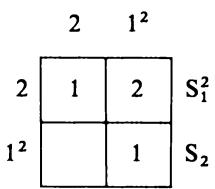
\includegraphics[keepaspectratio]{images/part001_666ab4c0.jpg}}

\pandocbounded{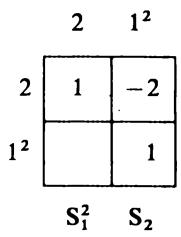
\includegraphics[keepaspectratio]{images/part001_442e375f.jpg}}

\(k = 3\)

3

2.1

\(1^{3}\)

3

1

3

6

\(S_{1}^{3}\)

2.1

1

3

\(S_{1}S_{2}\)

\(1^{3}\)

1

\(S_{3}\)

3 2.1 \(1^{3}\)\\
\pandocbounded{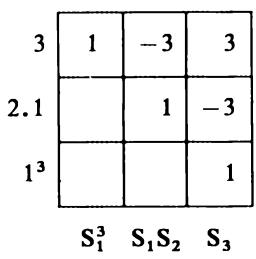
\includegraphics[keepaspectratio]{images/part001_fb1fe29f.jpg}}

\(k = 4\)

4

1

4

6

12

24

\(S_{1}^{4}\)

3.1

1

2

5

12

\(S_{1}^{2}S_{2}\)

\(2^{2}\)

1

2

6

\(S_{2}^{2}\)

\(2.1^{2}\)

1

4

\(S_{1}S_{3}\)

\(1^{4}\)

1

\(S_{4}\)

矩阵C

\pandocbounded{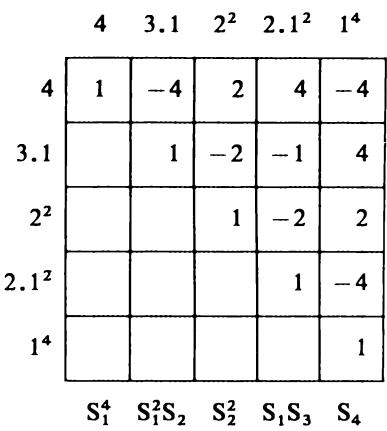
\includegraphics[keepaspectratio]{images/part001_bf35a948.jpg}}

\pandocbounded{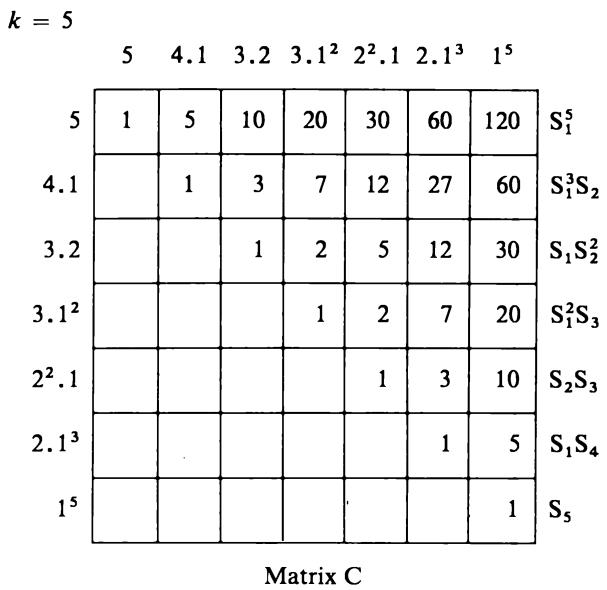
\includegraphics[keepaspectratio]{images/part001_7e862639.jpg}}

\pandocbounded{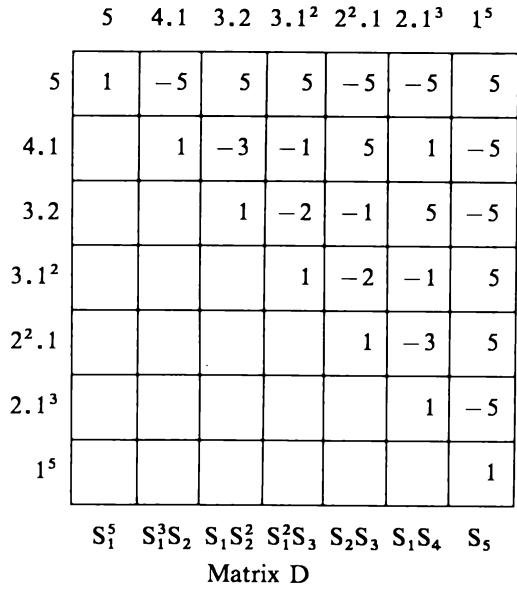
\includegraphics[keepaspectratio]{images/part001_eab66d56.jpg}}


\chapter{交换域}

除非另有明确说明，本章所考虑的所有域都是交换的；所有代数都是结合的且含单位元的，代数同态都是保单位的，代数的每个子代数都包含该代数的单位元。每当说一个域 K 包含在一个环 L 中（特别是包含在一个域中）而未作进一步说明时，即理解为 K 是 L 的一个子环；我们也说 K 是 L 的一个子域，或者（如果 L 是一个域）说 L 是 K 的一个扩域。

\section{素域。特征}

\subsection{素域}

有理整数环 Z 的分式域称为有理数域，记为 Q（I，第 117 页）。对每个素数 p，商环 \(\mathbf{Z}/(p)\) 是一个有限的 \(^{1}\) 、含 p 个元素的域，下文记为 \(F_{p}\) 。域 Q 是无限的，因为它包含 Z，因此不同构于任何域 \(F_{p}\) 。若 p 与 \(p'\) 是不同的素数，则域 \(F_{p}\) 与 \(F_{p'}\) 具有不同的基数，因此不同构。

定义 1. --- 一个域称为素域，如果它同构于 Q 或同构于某个域 \(F_{p}\) .

Q 的每个子域都包含环 Z，从而包含 Z 的分式域 Q；\(F_{p}\) 的每个子环都必然等于 \(F_{p}\) 。因此，素域的每个子域必然等于它本身（参见下面定理 1 的推论 2）。设 P 是一个素域，A 是一个环；若 f 与 \(f'\) 是 P 到 A 中的两个同态，则 \(x \in P\) （满足 \(f(x) = f'(x)\)）组成的集合是 P 的一个子域，因此根据上述结论必有 \(f = f'\) 。特别地，素域的唯一的自同态是恒等映射。

定理 1. --- 设 A 是一个环；假设 A 存在一个子域。则 A 有唯一的子域 P，它是一个素域。此外，P 包含在 A 的中心以及 A 的每个子域中。

设 K 为 A 的子域，C 为 A 的中心，并令 \(K' = K \cap C\) ；则 \(K'\) 是 A 的子域。设 f 为 Z 到 A 的唯一同态，p 为其核。A 的每个子环，特别是 \(K'\) ，包含 \(f(\mathbf{Z})\) ；因此理想 p 是素理想（I，第 116-117 页）。如果 \(\mathfrak{p} = (0)\) ，从 Z 到 \(K'\) 的同态 f 是单射；因此它（I，第 116 页）扩展为一个同构 \(\bar{f}\)（把 Q 映到 \(K'\) 的一个子域 P 上）。若 \(\mathfrak{p} \neq (0)\) ，存在一个严格正整数 p，使得 \(\mathfrak{p} = (p)\) （I，第 111 页）；如果我们有 p = ab，其中 a \textgreater{} 1 且 b \textgreater{} 1，这将意味着 \(a \notin p\) , \(b \notin p\) 且 \(ab \in p\) ，与 p 为素数的事实相矛盾。因此数 p 是素数，并且通过取商，f 定义了 \(F_p = Z/p\) 到 \(K'\) 的一个子域 P 上的一个同构。在这两种情形下，P 都是 A 的一个子域，且包含在 A 的中心 C 中，并且它是一个素域。设 L 是 A 的一个子域；则 \(P \cap L\) 是 P 的一个子域，由于 P 是素域，我们有 \(P \cap L = P\) ，从而 \(P \subset L\) 。若 \(P'\) 是 A 的一个子域且是素域，那么根据前面所述， \(P \subset P'\) ，从而 \(P = P'\) ，因为 \(P'\) 是素域。

推论 1. --- 设 K 是一个域。K 中存在唯一的素域子域，并且它是 K 的最小（在包含关系下）子域。

推论 2. --- 一个域是素域，当且仅当它不包含除自身以外的任何子域。

\subsection{环与域的特征}

我们仅当环 A 具有子域时才定义环 A 的特征。此时，设 f 是 Z 到 A 的唯一环同态，并设 n 是 Z 中生成作为 f 的核之理想的唯一正整数（I，第 111 页）；则整数 n 称为 A 的特征。

设 A 是一个已定义特征的环；则 A 不化为 0。由定理 1，A 中存在唯一的素域子域 P；我们称它为 A 的素子域。由定理 1 的证明，有以下两种可能：

\begin{enumerate}
\def\labelenumi{\alph{enumi})}
\item
  A 的特征为 0，P 同构于 Q，
\item
  \(\mathbf{A}\) 的特征是一个素数 \(p\)，\(\mathbf{P}\) 同构于 \(\mathbf{F}_p\) 。
\end{enumerate}

若 A 的特征为零，则存在 Q 到 A 的唯一环同态；其像为 A 的素子域，包含在 A 的中心中。因此，存在唯一的与环结构相容的 A 的 Q-代数结构。当 A 的特征为素数 p 时，把域 Q 替换为域 \(F_{p}\) 即得相应的性质。

命题 1. --- 设 A 是一个不化为 0 的环。

\begin{enumerate}
\def\labelenumi{\alph{enumi})}
\item
  为使 A 具有特征 0，必要且充分的是，映射 \(x \mapsto n \cdot x\)（A 到自身）对每个整数 \(n \neq 0\) 是双射。
\item
  设 \(p\) 为一个素数。为使 \(\mathbf{A}\) 具有特征 \(p\)，必要且充分的是 \(p \cdot x = 0\) 对所有 \(x \in \mathbf{A}\) 成立。
\end{enumerate}

设 \(f\) 是 \(\mathbf{Z}\) 到 \(\mathbf{A}\) 中的唯一同态；我们有 \(n \cdot x = f(n)x\)，对每个整数 \(n\) 及每个 \(x\) （在 \(\mathbf{A}\) 中）。为使 \(\mathbf{A}\) 具有特征 0，必要且充分的是 \(f\) 可扩展为 \(\mathbf{Q}\) 到 \(\mathbf{A}\) 中的一个同态，即 \(f(n)\) 在 \(\mathbf{A}\) 中可逆，对每个 \(n \neq 0\)（I，第 113 页）；这就证明了 \(a\) )。类似地，为使 \(\mathbf{A}\) 具有特征 \(p\)，必要且充分的是 \(f\) 零化 \(p\mathbf{Z}\)，即 \(f(p) = 0\)，或者也即 \(p \cdot x = 0\) 对所有 \(x \in \mathbf{A}\) 成立；这就证明了 \(b\) 。

设 A 为一个不一定交换的域。A 的中心是一个（交换）域；因此 A 的特征和素子域是有定义的。

注记。--- 1) 设 A 与 A' 为两个不化为 0 的环。假设 A 的特征已定义，并且存在一个从 A 到 A' 的同态 u。A 的素子域在 u 下的像是 A' 的一个子域 P'，与 P 同构，因此也是素域。由此可知 A' 的特征已定义，并且等于 A 的特征。若 A 与 A' 的特征为 0（相应地， \(p \neq 0\) ），映射 u 是 Q 上代数的一个同态（相应地， \(F_{p}\) 上代数的同态）。

\begin{enumerate}
\def\labelenumi{\arabic{enumi})}
\setcounter{enumi}{1}
\item
  注 1 表明，若 A 是特征为 0 的环（相应地， \(p \neq 0\) ），则任何以 A 为子环的环 A'，或 A 关于双边理想 \(\mathfrak{a} \neq \mathbf{A}\) 的任何商环，也具有同样的性质。特别地，若 K 是域，则 K 的每个子域和 K 的每个扩域都与 K 具有相同的特征。
\item
  设 A 是域 K 上的一个不化为 0 的代数。由于映射 \(\lambda \mapsto \lambda \cdot 1\)（从 K 到 A）是环同态，注记 1 表明 A 的特征有定义且等于 K 的特征。
\item
  由于域 \(\mathbf{Q}\) 是无限的，每个特征为0的环都是无限的；因此，每个有限域都有非零特征。
\item
  设 A 是一个不化为 0 的环，其加法群是一个无挠 Z-模，并令 \(B = Q \otimes_{Z} A\) 。映射 \(x \mapsto 1 \otimes x\)（从 A 到 B）是单射（II，第 314 页），因此 A 同构于一个特征为 0 的环的子环。
\end{enumerate}

\subsection{\texorpdfstring{特征为 \(p\) 的交换环}{特征为 p 的交换环}}

在本节及下一节中，p 表示一个素数。

定理 2. --- 设 A 是一个特征为 p 的交换环。映射 \(a \mapsto a^{p}\) 是环 A 的一个自同态，即我们有关系式

\[
(a + b) ^ {p} = a ^ {p} + b ^ {p}\tag{1}
\]

\[
(a b) ^ {p} = a ^ {p} b ^ {p}\tag{2}
\]

对 A 中的 \(a, b\) 成立。

公式 (2) 由 A 的交换性得出。为证明 (1)，我们使用二项式公式 \((a + b)^p = a^p + b^p + \sum_{i=1}^{p-1} \binom{p}{i} \cdot a^ib^{p-i}\)；由于 \(p \cdot x = 0\) 对所有 \(x \in \mathbf{A}\) 成立，只需证明以下引理：

引理 1. --- 设 \(p\) 是一个素数，\(i\) 是从 1 到 \(p - 1\) 范围内的一个整数，则二项式系数 \(\binom{p}{i}\) 是一个可被 \(p\) 整除的整数。

我们对 \(i\) 作归纳论证，情形 \(i = 1\) 由公式 \(\binom{p}{1} = p\) 直接得出。假设 \(2 \leqslant i \leqslant p - 1\) 且 \(\binom{p}{i - 1}\) 能被 \(p\) 整除。则整数 \(i\binom{p}{i} = (p - i + 1)\binom{p}{i - 1}\) 属于素理想 \(p\mathbf{Z}\)（\(\mathbf{Z}\) 的素理想）；由于 \(i \notin p\mathbf{Z}\)，我们有 \(\binom{p}{i} \in p\mathbf{Z}\)，引理得证。

设 A 是特征为 p 的交换环，f 为一个整数 \(\geqslant0\)。由定理 2，我们通过对 f 的归纳法推出，映射 \(a\mapsto a^{p^{f}}\) 是环 A 的一个自同态。特别地，我们有关系式

\[
(a _ {1} + \dots + a _ {n}) ^ {p ^ {f}} = a _ {1} ^ {p ^ {f}} + \dots + a _ {n} ^ {p ^ {f}}\tag{3}
\]

对 A 中任意的 \(a_{1},\ldots,a_{n}\) 成立。映射 \(a\mapsto a^{p}\) 有时称为 A 的弗罗贝尼乌斯自同态。取 \(\mathbf{A}=\mathbf{F}_{p}\) 且 \(a_{i}=1\)，我们由 (3) 得到关系式：

\[
n ^ {p ^ {f}} \equiv n \mod p (n \in \mathbf {Z}, f \in \mathbf {N}).\tag{4}
\]

对 A 的每个子集 S，我们用 \(S^{p^{f}}\) 表示 A 中形如 \(x^{p^{f}}\)（其中 \(x \in S\)）\(^{1}\) 的元素所组成的集合。特别地，若 K 是 A 的一个子环，则集合 \(K^{p^{f}}\) 是 A 的一个子环。若 K 是 A 的一个子环且 S 是 A 的一个子集，我们用 K{[}S{]} 表示由 \(K \cup S\) 生成的 A 的子环；当 A 是一个域时，我们用 \(\mathrm{K}(S)\) 表示 K{[}S{]} 的分式域，即由 \(K \cup S\) 生成的 A 的子域。

命题 2. --- 设 A 是特征为 p 的交换环，K 是 A 的一个子环，S 是 A 的一个子集，f 是一个正整数。

\begin{enumerate}
\def\labelenumi{\alph{enumi})}
\item
  我们有 \(\mathbf{K}[\mathbf{S}]^{p^f} = \mathbf{K}^{p^f}[\mathbf{S}^{p^f}]\)，且若 \(\mathbf{A}\) 是一个域，则 \(\mathbf{K}(\mathbf{S})^{p^f} = \mathbf{K}^{p^f}(\mathbf{S}^{p^f})\) 。
\item
  若 K-模 K{[}S{]} 由 A 的元素组成的族 \((a_{i})_{i\in I}\) 生成，则 K-模 \(K[S^{p^{f}}]\) 由族 \((a_{i}^{p^{f}})_{i\in I}\) 生成。
\end{enumerate}

由于 K{[}S{]} 是 A 中由 K ∪ S 生成的子环，它的像 K{[}S{]} \(^{p^{f}}\) （在环 A 的自同态 \(\pi: a \mapsto a^{p^{f}}\) 下）是 A 中由 K ∪ S 的像 K \(^{p^{f}}\) ∪ S \(^{p^{f}}\) （在 \(\pi\) 下）生成的子环，因此 K{[}S{]} \(^{p^{f}}\) = K \(^{p^{f}}\) {[}S \(^{p^{f}}\) {]}。域的情形类似处理；这就证明了 a)。

显然，族 \((a_i^{p^f})_{i\in I}\) 生成 \(\mathbf{K}^{p^f}\) -模 \(\mathbf{K}[\mathbf{S}]^{p^f}\) 。K-模 \(\mathbf{K}[\mathbf{S}^{p^f}]\) 由形如 \(x_1^{p^f}\ldots x_n^{p^f} = (x_1\ldots x_n)^{p^f}\)（其中 \(x_1,\ldots ,x_n\) 在 S 中任意）的乘积生成，因此也由集合 \(\mathbf{K}[\mathbf{S}]^{p^f}\) 生成。断言 b) 直接由此得出。

\(^{1}\) 当然，集合 \(S^{p^{f}}\) 不应与 \(p^{f}\) 个都等于 S 的集合的集合积相混淆，也不应与属于 S 的 \(p^{f}\) 个元素的乘积组成的集合相混淆。

\subsection{\texorpdfstring{特征为 \(p\) 的完全环}{特征为 p 的完全环}}

定义 2. --- 一个特征为 \(p \neq 0\) 的环 A 称为完全环，如果它是交换的且映射 \(a \mapsto a^p\) 是双射的。

如果环 A 是特征 p 的完全环，映射 \(a \mapsto a^{p^{f}}\) 对每个整数 \(f \geqslant 0\) 是环 A 的自同构；逆自同构记为 \(a \mapsto a^{1/p^{f}}\) 或 \(a \mapsto a^{p^{-f}}\)，并且 A 的子集 S 在该自同构下的像记为 \(S^{1/p^{f}}\) 或 \(S^{p^{-f}}\) 。显然 \((a^{p^{e}})^{p^{f}} = a^{p^{e+f}}\) 对所有 \(a \in A\) 以及任意整数 e 和 f（无论其符号如何）成立。

设 A 是特征为 p 的交换环。对每个整数 \(f \geqslant 0\)，用 \(n_{f}\) 表示环 A 的自同态 \(a \mapsto a^{p^{f}}\) 的核。则 \((\mathfrak{n}_{f})_{f \geqslant 0}\) 是 A 的理想的一个递增序列；由于每个正整数都被 p 的某个幂所控制，理想 \(n = \bigcup_{f \geqslant 0} n_{f}\) 由 A 的所有

幂零元素组成。特别地，若 A 是完全的，则 A 的每个幂零元素都为零。

定义 3. --- 设 A 是一个特征为 \(p \neq 0\) 的交换环。所谓 A 的完全闭包，我们指的是一个对 \((\hat{\mathbf{A}}, u)\)，其中 \(\hat{\mathbf{A}}\) 是特征为 \(p\) 的完全环，且 \(u\) 是 A 到 \(\hat{\mathbf{A}}\) 中的一个同态，满足如下泛性质：

（PC）若 B 是特征为 p 的完全环，且 v 是从 A 到 B 的同态，则存在唯一的同态 h（从 \(\hat{A}\) 到 B 中），使得 \(v = h \circ u\) 。

泛性质（PC）立即蕴含完全闭包的唯一性，其含义如下：若 \((\hat{\mathbf{A}}, u)\) 与 \((\hat{\mathbf{A}}', u')\) 是 A 的两个完全闭包，则存在唯一的、把 \(\hat{A}\) 映到 \(\hat{A}'\) 上的同构 h，使得 \(u' = h \circ u\) （参见 E，IV，第 23 页）。我们现在来建立完全闭包的存在性：

定理 3. --- 设 A 是一个特征为 \(p \neq 0\) 的交换环。则 A 存在一个完全闭包 \((\hat{\mathbf{A}}, u)\)。此外，\(u\) 的核是 A 的所有幂零元素组成的集合，并且对于每个 \(x \in \hat{\mathbf{A}}\)，存在一个整数 \(n \geqslant 0\)，使得 \(x^{p^n} \in u(\mathbf{A})\) 。

对每个整数 \(n \geqslant 0\)，令 \(\mathbf{A}_n = \mathbf{A}\)；当 \(m \geqslant n\) 时，我们定义一个同态 \(\pi_{m,n}\)（从 \(\mathbf{A}_n\) 到 \(\mathbf{A}_m\) 中），由 \(\pi_{m,n}(a) = a^{p^{m-n}}\) 给出。这样我们得到环的一个正向系统 \((\mathbf{A}_n, \pi_{m,n})\)（I，第 120 页）；设 \(\hat{\mathbf{A}}\) 为该系统的正向极限，\(u_n\) 为 \(\mathbf{A}_n = \mathbf{A}\) 到 \(\hat{\mathbf{A}}\) 中的典范同态；我们还令 \(u = u_0\)。根据正向极限的构造，核 \(n\) （\(u\) 的）是 A 到 A 中的同态 \(\pi_{n,0}: a \mapsto a^{p^n}\) 的核的并集，因此它由 A 的所有幂零元素组成。环 \(\hat{A}\) 根据 V 第 3 页的注记 1 是特征为 p 的交换环。

环 \(\hat{\mathbf{A}}\) 是子环的递增序列 \((u_n(\mathbf{A}))_{n\geq 0}\) 的并集。我们有 \(u_{n}(\mathbf{A})^{p^{n}} = \mathbf{A}\)；因此对每个 \(x\in \hat{\mathbf{A}}\)，存在一个整数 \(n\geqslant 0\)，使得 \(x^{p^n}\in u(\mathbf{A})\)。我们还有 \(u_{n}(\mathbf{A}) = u_{n + 1}(\mathbf{A})^{p}\)，从而 \(\hat{\mathbf{A}}^p = \hat{\mathbf{A}}\)。设 \(x\in \hat{\mathbf{A}}\) 使得 \(x^{p} = 0\)；选择一个整数 \(n\geqslant 1\) 和一个元素 \(a\in \mathbf{A}\)，使得 \(x = u_{n}(a)\)。于是我们有 \(u_{n - 1}(a) = u_n(a)^p = 0\)；根据正向极限的定义，存在一个整数 \(m\geqslant n\)，使得 \(\pi_{m - 1,n - 1}(a) = 0\)，即 \(a^{p^{m - n}} = 0\)。因此我们有 \(\pi_{m,n}(a) = 0\)，从而 \(u_{n}(a) = 0\)，即 \(x = 0\)。因此环 \(\hat{\mathbf{A}}\) 是特征为 \(p\) 的完全环。

设 \(v\) 是 \(A\) 到完全环 \(B\)（特征为 \(p\)）中的一个同态。对每个整数 \(n \geqslant 0\)，映射 \(b \mapsto b^{p^n}\) 是 \(B\) 的一个自同构，因此存在一个同态 \(v_n\) （从 \(A_n = A\) 到 \(B\) 中），它由 \(v(a) = v_n(a)^{p^n}\) 刻画。于是我们有 \(v_m \circ \pi_{m,n} = v_n\)，对 \(m \geqslant n \geqslant 0\)；根据正向极限的定义，存在一个同态 \(h\) （从 \(\hat{A}\) 到 \(B\) 中），使得 \(v_n = h \circ u_n\) 对所有 \(n \geqslant 0\) 成立；特别地，我们有 \(v = v_0 = h \circ u_0 = h \circ u\)。最后设 \(h'\) 是 \(\hat{A}\) 到 \(B\) 中的一个同态，使得 \(h' \circ u = v\)。设 \(x \in \hat{A}\)；如我们所见，存在一个整数 \(n \geqslant 0\) 和一个元素 \(a \in A\)，使得 \(x^{p^n} = u(a)\)。于是我们有

\[
h (x) ^ {p ^ {n}} = h (u (a)) = v (a) = h ^ {\prime} (u (a)) = h ^ {\prime} (x) ^ {p ^ {n}},
\]

且由于 B 是完全的，我们得到 \(h(x) = h'(x)\)。于是我们有 \(h' = h\)，这就完成了 \((\hat{\mathbf{A}}, u)\) 是 A 的完全闭包的证明。

命题 3. --- 设 B 是特征为 p 的完全环，A 是 B 的一个子环。记 \(A^{p^{-\infty}} = \bigcup_{f \geqslant 0} A^{p^{-f}}\)，并用 j 表示 A 到

\(\mathbf{A}^{p^{-\infty}}\) 中的典范单射。则 \(\mathbf{A}^{p^{-\infty}}\) 是 \(\mathbf{B}\) 的包含 \(\mathbf{A}\) 的最小完全子环，且 \((\mathbf{A}^{p^{-\infty}}, j)\) 是 \(\mathbf{A}\) 的一个完全闭包。

对每个整数 \(f \in \mathbf{Z}\)，用 \(\pi_f\) 表示自同构 \(b \mapsto b^{p^f}\) （\(\mathbf{B}\) 的）。子环序列 \(\pi_{-f}(\mathbf{A})\) （在 \(\mathbf{B}\) 中）（对 \(f \geqslant 0\)）是递增的，其并集 \(\mathbf{A}^{p^{-\infty}}\) 因而是 \(\mathbf{B}\) 的一个子环。我们有 \(\pi_1(\mathbf{A}^{p^{-\infty}}) = \bigcup_{f \geqslant 0} \pi_{-(f-1)}(\mathbf{A}) = \mathbf{A}^{p^{-\infty}}\)，因此

\(A^{p^{-\infty}}\) 是 B 的一个完全子环。最后令 \(B_0\) 是 B 的一个完全子环且包含 A；对每个整数 \(f \geqslant 0\)，我们有 \(\pi_{-f}(A) \subset \pi_{-f}(B_0) = B_0\)，从而 \(A^{p^{-\infty}} \subset B_0\) 。

如果 \(v\) 是 \(\mathbf{A}\) 到完全环 \(\mathbf{B}'\)（特征为 \(p\)）中的一个同态，则对每个整数 \(f \geqslant 0\)，我们可以定义一个同态 \(h_f\) （从 \(\pi_{-f}(\mathbf{A})\) 到 \(\mathbf{B}'\) 中），由 \(h_f(\pi_{-f}(a)) = v(a)^{p^{-f}}\)（对所有 \(a \in \mathbf{A}\)）给出。我们立刻看到 \(h_{f + 1}\) 与 \(h_f\) 在 \(\pi_{-f}(\mathbf{A})\) 上一致；因此存在一个同态 \(h\) （从 \(\mathbf{A}^{p^{-\infty}}\) 到 \(\mathbf{B}'\) 中），它把 \(h_f\) 诱导在 \(\pi_{-f}(\mathbf{A})\) 上（对所有 \(f \geqslant 0\)），特别地，\(h\) 扩张 \(h_0 = v\)。若 \(h'\) 是 v 的另一个扩张——扩张为 \(A^{p^{-\infty}}\) 到 B 中的同态——则等式 \(h' = h\) 可按定理 3 的证明中的方法建立。

\subsection{域的特征指数。完全域}

设 K 为一个域。K 的特征指数指的是这样一个整数：若 K 的特征为 0，它等于 1；若特征非零，它等于 K 的特征。

命题 4. --- 设 K 是特征指数为 q 的域。对每个整数 \(f \geqslant 0\)，映射 \(x \mapsto x^{q^{f}}\) 是 K 到它的一个子域上的同构（记作 \(K^{q^{f}}\)）。

当 \(q \neq 1\) 时这由定理 2 得出，而当 \(q = 1\) 时是平凡的。

同样地，可以把命题 2 推广到 A 是特征指数为 q 的域的情形，q = 1 的情形是平凡的。

定义 4. --- 一个特征指数为 q 的域 K 称为完全域，如果 \(K^{q} = K\) 。当 \(K^{q} \neq K\) 时，称 K 为非完全域。

根据这一定义，一个域是完全的，如果它的特征为 0，或者它是定义 2 意义下特征为 \(p \neq 0\) 的完全环。如果 \(\mathbf{K}\) 是一个特征为 \(p \neq 0\) 的域，且 \((\hat{\mathbf{K}}, u)\) 是 \(\mathbf{K}\) 的一个完全闭包，则根据命题 3（V，第 6 页），\(\hat{\mathbf{K}}\) 是一个域，且 \(u\) 是 \(\mathbf{K}\) 到 \(\hat{\mathbf{K}}\) 的某个子域上的一个同构。通常把 \(\mathbf{K}\) 与它在 \(u\) 下的像在 \(\hat{\mathbf{K}}\) 中等同起来，于是我们有 \(\hat{\mathbf{K}} = \mathbf{K}^{p^{-\infty}}\)（命题 3）。

设 K 为特征为 0 的域；则 K 的特征指数为 1。按约定，记号 \(x^{q^{-f}}\) 与 \(S^{q^{-f}}\) 分别表示 x 和 S（其中 x 是 K 的元素，S 是 K 的子集）。特别地，我们令 \(K^{q^{-\infty}} = K\)，并且约定取 K 的完全闭包为 K 本身。

命题 5. --- 若 K 是特征为 0 的域，或者是有限域*或代数闭域*，则它是完全域。特别地，每个素域都是完全域。

假设 K 的特征为 \(p \neq 0\) 。若 K 为有限域，则子域 \(K^{p}\) 与 K 具有相同的基数，从而 \(K^{p} = K\)。* 若 K 是代数闭的，则多项式 \(X^{p} - a\) 对每个 \(a \in K\)（V，第 20 页，定义 1）在 K 中有一个根 x，因此 \(x^{p} = a\)，于是 \(K^{p} = K\)。* 最后，素域的特征为 0 或有限。

设 \(K_{0}\) 是特征为 \(p \neq 0\) 的域，\(\mathbf{K} = \mathbf{K}_{0}(\mathbf{X})\) 是不定元 X 上 \(K_{0}\) 上的有理分式域。则 K 是非完全域，因为不存在 K 的元素 \(u(\mathbf{X})/v(\mathbf{X})\)（u，v 是 \(K_{0}[\mathbf{X}]\) 中的多项式），使得 \((u(\mathbf{X})/v(\mathbf{X}))^{p} = \mathbf{X}\)。把该关系写成 \(u(\mathbf{X})^{p} = \mathbf{X}v(\mathbf{X})^{p}\) 的形式并比较两边的次数即可看出这一点。

\subsection{具有零微分的多项式的刻画}

命题 6. --- 设 K 为一个交换环，A 为多项式代数 \(K[X_{i}]_{i \in I}\)，S 为 A 中满足 dF = 0 的元素 F 的集合。

\begin{enumerate}
\def\labelenumi{\alph{enumi})}
\item
  如果 \(\mathbf{K}\) 是特征为 0 的环，则 \(\mathbf{S} = \mathbf{K}\) 。
\item
  如果 \(\mathbf{K}\) 是特征为 \(p \neq 0\) 的环，则 \(\mathbf{S} = \mathbf{K}[\mathbf{X}_i^p]_{i \in I}\)；此外如果 \(\mathbf{K}\) 是完全环，则 \(\mathbf{K} = \mathbf{A}^p\) 。
\end{enumerate}

映射 \(F \mapsto dF\)（从 A 到 A 的 K-微分形式模 \(\Omega_{\mathbf{K}}(\mathbf{A})\) 中）是 K-线性的，并且满足关系

\[
d \left(\mathrm{FF} ^ {\prime}\right) = \mathrm{F} \cdot d \mathrm{F} ^ {\prime} + \mathrm{F} ^ {\prime} \cdot d \mathrm{F}
\]

（III，第 569 页）。因此 S 是一个子代数。

当 K 的特征为 \(p \neq 0\) 时，令 \(T = K[X_{i}^{p}]_{i \in I}\)；于是若 K 是完全的，我们有 \(T = A^{p}\)（V，第 4 页，命题 2）；此外，我们有 \(d(X_{i}^{p}) = pX_{i}^{p-1}\)，\(dX_{i} = 0\) 对所有 \(i \in I\) 成立，因此 A 的子代数 S 包含 T。若 K 的特征为 0，我们令 T = K，并且仍然得到 \(T \subset S\) 。还需证明 S 包含于 T。

对每个有限子集 \(J\) （属于 \(I\)），令 \(A_{J}\) 为 \(A\) 的由族 \((X_{j})_{j\in J}\) 生成的子代数。我们有 \(A_{\emptyset} = K\) 且 \(A = \bigcup_{J\in I}A_{J}\)；因此只需证明

关系 \(S \cap A_{J} \subset T\)，我们将通过对 J 的基数进行归纳来证明。因此，设 J 是 I 的一个有限子集，使得 \(S \cap A_{J} \subset T\)，设 i 是 I - J 的一个元素，且 \(J' = J \cup \{i\}\) 。\(A_{J}\) 的每个元素 F 都可以以唯一的方式写成形式

\[
\mathrm{F} = \sum_ {n = 0} ^ {\infty} \mathrm{F} _ {n} \cdot \mathrm{X} _ {i} ^ {n},\tag{5}
\]

其中 \(\mathbf{F}_n\in \mathbf{A}_{\mathrm{J}}\) 对所有 \(n\geqslant 0\)，然后

\[
d \mathrm{F} = \sum_ {n = 0} ^ {\infty} \mathrm{X} _ {i} ^ {n} \cdot d \mathrm{F} _ {n} + \sum_ {n = 0} ^ {\infty} n \mathrm{X} _ {i} ^ {n - 1} \mathrm{F} _ {n} \cdot d \mathrm{X} _ {i}.\tag{6}
\]

假设 F 属于 S；族 \((d\mathbf{X}_{r})_{r\in I}\) 是 A-模 \(\Omega_{\mathrm{K}}(\mathbf{A})\) 的一组基（III，第 570 页），且 \(dF_{n}\) 是微分 \(dX_{j}\)（对 \(j\in J\)）的线性组合，因为 \(F_{n}\in A_{J}=K[X_{j}]_{j\in J}\) 。由 (6) 我们则有 \(dF_{n}=0\) 且 \(nF_{n}=0\)，对每个整数 \(n\geqslant0\)。由归纳假设，\(F_{n}\in T\) 对所有 n 成立，因为 \(dF_{n}=0\) 。

\begin{enumerate}
\def\labelenumi{\alph{enumi})}
\item
  若 K 的特征为 0，则我们有 \(nF_{n} = 0\) 对所有 \(n \geqslant 1\) 成立，从而由命题 1（V，第 2 页）得 \(F_{n} = 0\)；因此我们有 \(F = F_{0}\)，从而 \(F \in T\) 。
\item
  如果 \(\mathbf{K}\) 的特征为 \(p \neq 0\)，则 \(\mathbf{A}\) 是域 \(\mathbf{F}_p\) 上的代数，且关系 \(n\mathrm{F}_n = 0\) 蕴含 \(\mathbf{F}_n = 0\)，对每个整数 \(n\) （不被 \(p\) 整除）成立。因此我们有 \(\mathbf{F} = \sum_{m=0}^{\infty} \mathbf{F}_{mp} \mathbf{X}_i^{mp}\)，从而 \(\mathbf{F} \in \mathbf{T}\) 。
\end{enumerate}

注记。--- 当 K 的加法群无挠时，我们仍有 S = K；这可由上述证明或 V 第 3 页的注记 5 得出。

推论。--- 设 K 为一个域，F(X) 是系数在 K 中的多项式，其导数 F'(X) 为零。

\begin{enumerate}
\def\labelenumi{\alph{enumi})}
\item
  如果 \(\mathbf{K}\) 的特征为 0，则 \(\mathbf{F} \in \mathbf{K}\) 。
\item
  如果 \(\mathbf{K}\) 的特征为 \(p \neq 0\)，则存在一个多项式 \(\mathbf{G}(\mathbf{X})\)，使得 \(\mathbf{F}(\mathbf{X}) = \mathbf{G}(\mathbf{X}^p)\) 。
\end{enumerate}

因为我们有 \(d\mathbf{F} = \mathbf{F}' \cdot d\mathbf{X} = 0\) 。

\section{扩张}

\subsection{扩张的结构}

定义 1. --- 设 K 是一个域。所谓 K 的一个扩张，我们指的是一个 K-代数，其底环是一个域。所谓扩张 E 的一个子扩张（或 K-子扩张），我们指的是 E 的一个子 K-代数，且其本身是一个域。

设 E 是 K 的一个扩张。映射 \(u: \lambda \mapsto \lambda \cdot 1\)（从 K 到 E）是一个环同态；由 I，第 115 页，u 诱导出 K 到 E 的子域 \(u(\mathbf{K})\) 上的一个同构。

反之，若 K、E 是域且 u 是 K 到 E 的一个同态，则 u 在 E 上定义了 K 的一个扩张结构（III，第 433 页）。滥用语言时，有时称 \((E, u)\) 是 K 的一个扩张。

一个扩张称为平凡的，如果 \(u(\mathbf{K}) = \mathbf{E}\)，即如果 E 是 K 上的一维向量空间。

设 L 是 K 的一个扩张域。当我们把 L 视为 K 的扩张时，我们指的是 K 的扩张 \((L, j)\)，其中 j 是 K 到 L 的典范单射，或者也可以指带有相应 K-代数结构的 L。此时 L 的子扩张就是 K 与 L 之间的中间域，即包含 K 的 L 的子域。若 \(L'\) 是 K 的另一个扩张域，则 L 到 \(L'\) 的一个 K-同态就是 L 到 \(L'\) 的一个满足 \(f(x) = x\)（对所有 \(x \in K\)）的同态 f。我们注意到，若 f 是域 L 的任一自同态，则 L 中在 f 下不变的元素之集是 L 的一个子域 \(K'\)，且 f 此时是 L 的 \(K'\)-自同态。

特别地，设 P 是域 L 的素子域。我们可以将 L 视为 P 的扩张，并且 L 的每个自同态此时都是 P-自同态。

\pandocbounded{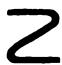
\includegraphics[keepaspectratio]{images/part001_5fd131d7.jpg}}

设 \((\mathrm{E}, u)\) 是 K 的一个扩张；由于 u 定义了 K 到 E 的某个子域 \(K_{1}\) 上的同构，通常不难通过 u 把 K 与 \(K_{1}\) 等同起来。有一种情况我们不能允许这种等同，即当 K = E 且 u 因此是 K 的自同态时；最常见的是 u 为 K 的自同构，或映射 \(u \mapsto u^{p}\)（当域 K 的特征 \(\neq 0\) 时）。

显然，K 的每个扩张都同构于一个扩张 \((L, j)\) ，其中 L 是包含 K 作为子域的域，j 是 K 到 L 的典范嵌入。

\subsection{扩张的次数}

设 A 是域 K 上的代数。它特别是 K 上的向量空间；这个向量空间的维数称为 A 在 K 上的次数，记作 \([A:K]\) （II，第 293 页）。根据定义， \([A:K]\) 因此是 A 在 K 上的任意基的基数。这个定义特别适用于 K 的扩张的情形。

次数为 1 的扩张是平凡的。次数为 2（分别为 3 等）的扩张称为二次（分别为三次等）扩张。有限次数的扩张有时被滥用语言地称为有限扩张。

定理 1. --- 设 E 是 K 的扩张，A 是 E 上的代数。那么我们有 \([A:K]=[A:E]\)。\([E:K]\)。特别地，若 F 是 E 的扩张，我们有

\[
[ \mathbf {F}: \mathbf {K} ] = [ \mathbf {F}: \mathbf {E} ]. [ \mathbf {E}: \mathbf {K} ].\tag{1}
\]

该定理只是 II，第 222 页，命题 25 的一个特例；更确切地说，如果 \((a_{\lambda})_{\lambda \in L}\) 是 A 在 E 上的一组基，且 \((b_{\mu})_{\mu \in M}\) 是 E 在 K 上的一组基，则族 \((a_{\lambda}b_{\mu})_{(\lambda ,\mu)\in L\times M}\) 是 A 在 K 上的一组基。

推论 1. --- 设 K、E、F 为三个域，使得 \(K \subset E \subset F\) 且 \([F:K]\) 是有限的。则次数 \([E:K]\) 与 \([F:E]\) 是 \([F:K]\) 的因子。

如果次数 \([F:K]\) 是素数，则 F 除 K 和 F 外没有其他子扩张。但要注意，当 \([F:K]\) 不是素数时，不一定存在 F 的除 K 和 F 以外的子扩张（参见 V，第 146 页，习题 1）。

推论 2. --- 设 K、E 和 F 为三个域，使得 \(K \subset E \subset F\) 。假设 \([F:K]\) 是有限的，则关系 \([E:K] = [F:K]\) 等价于 E = F，且关系 \([F:E] = [F:K]\) 等价于 E = K。

因为若 L 是 \(L'\) 的一个扩张域，则 \([L:L'] = 1\) 等价于 \(L' = L\) 。

命题 1. --- 设 A 是域 K 上的一个有限次代数。若一个元素 \(a \in \mathbf{A}\) 在 A 中不是左（相应地，右）零因子，则它在 A 中可逆。

因为 A 在 K 上的向量空间按假设是有限维的，且线性映射 \(x \mapsto ax\)（相应地 \(x \mapsto xa\)）（从 A 到 A）是单射；因此它是双射（II，第 298 页，推论），从而（I，第 16 页，注记）a 在 A 中可逆。

推论。--- 设 A 是域 K 上的一个有限次交换代数。若 A 是整环，则它是一个域。

\subsection{添加}

设 E 是域 K 的一个扩张。给定一族 E 中的元素 \(\mathbf{x} = (x_{i})_{i \in I}\)，我们用 \(\mathrm{K}(x_{i})_{i \in I}\)（或 \(\mathrm{K}(\mathbf{x})\)，或也记作 \(\mathrm{K}(x_{1}, \ldots, x_{n})\)，当 I 是 N 中的区间 {[}1, n{]} 时）表示包含该族成员 \((x_{i})\) 的最小子扩张；我们说 \(\mathrm{K}(x_{i})_{i\in I}\) 是通过把族 \((x_{i})_{i\in I}\) 中的元素添加到 K 上而得到的，并且该族 \((x_{i})_{i\in I}\)（或其元素的集合）是 \(\mathrm{K}(x_{i})_{i\in I}\) 关于 K（或在 K 上）的生成族。域 \(\mathrm{K}(x_{i})_{i\in I}\) 仅依赖于族 \((x_{i})_{i\in I}\) 的元素集合 A；我们也把它记作 \(\mathrm{K}(\mathrm{A})\) 。特别地，我们有 \(\mathrm{K}(\mathrm{E})=\mathrm{E}\) 且 \(\mathrm{K}(\emptyset)=\mathrm{K} \cdot 1\) 。以上所述特别适用于 E 为包含 K 作为子域的域的情形。

\pandocbounded{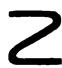
\includegraphics[keepaspectratio]{images/part001_724f36f3.jpg}}

应当注意，A 一般不构成代数 \(\mathbf{K}(\mathbf{A})\) 的生成集，换言之，\(\mathbf{K}(\mathbf{A}) \neq \mathbf{K}[\mathbf{A}]\) 。* 然而我们将看到，\(\mathbf{K}(\mathbf{A}) = \mathbf{K}[\mathbf{A}]\)（当 \(\mathbf{K}(\mathbf{A})\) 是 \(\mathbf{K}\) 的一个代数扩张时；V，第 18 页，推论 1）。*

命题 2. --- 若 M 和 N 是域 K 的一个扩张中的任意两个子集，则 \(\mathbf{K}(\mathbf{M} \cup \mathbf{N}) = \mathbf{K}(\mathbf{M})(\mathbf{N}) = \mathbf{K}(\mathbf{N})(\mathbf{M})\) 。

因为 \(\mathbf{K}(\mathbf{M} \cup \mathbf{N})\) 包含 \(\mathbf{K}(\mathbf{M})\) 与 \(\mathbf{N}\)，因此包含 \(\mathbf{K}(\mathbf{M})(\mathbf{N})\)；由于 \(\mathbf{K}(\mathbf{M})(\mathbf{N})\) 是一个包含 \(\mathbf{K} \cup \mathbf{M} \cup \mathbf{N}\) 的域，它包含 \(\mathbf{K}(\mathbf{M} \cup \mathbf{N})\)，由此得出该命题。

我们有时会写 \(\mathbf{K}(\mathbf{M},\mathbf{N})\) 以代替 \(\mathbf{K}(\mathbf{M}\cup \mathbf{N})\) 。

注记. --- 设P是域E的素子域（V，第2页）；对于E的每个子集A，P(A)是E中包含A的最小子域。特别地，若K是E的一个子域，则有P(K ∪ A) = K(A)。若K和K'是E的两个子域，则我们有P(K ∪ K') = K(K') = K'(K)；这个域是E中包含K或K'的最小子域，或者说是E的子域集合（按包含关系排序）中K和K'的上确界；我们有时称这个域为K和K'在E中生成的域。

命题 3. --- 设 F 是域 E 的一族子域，关于关系 ⊂ 是定向的。F 中各域的并 L 是一个域。

因为如果 \(x\) 与 \(y\) 是 \(L\) 的两个元素，则存在两个域 \(R, S\) （属于 \(\mathcal{F}\)），使得 \(x \in R\), \(y \in S\)；设 \(T\) 是 \(\mathcal{F}\) 中包含 \(R\) 与 \(S\) 的一个域；则 \(x \in T\), \(y \in T\)，因此 \(x + y\), \(xy\) 与 \(x^{-1}\)（若 \(x \neq 0\)）属于 \(T\)，从而属于 \(L\) 。

推论。--- 设 E 是域 K 的扩域，且 A ⊂ E。域 K(A) 是域 K(F) 的并集，其中 F 遍历 A 的所有有限子集所成的集合。

因为域的集合 \(\mathbf{K}(\mathbf{F})\) 按关系 \(\subset\) 定向，因为 \(F \subset F'\) 蕴含 \(\mathbf{K}(\mathbf{F}) \subset \mathbf{K}(\mathbf{F}')\) 。这些域的并集 L 因而是包含 \(K \cup A\) 且包含于 \(\mathbf{K}(\mathbf{A})\) 中的域，从而与 \(\mathbf{K}(\mathbf{A})\) 相同。

定义 2. --- 域 K 的扩张 E 称为有限生成的，如果它有一个有限生成族。它称为单生成的，如果存在 E 中的 x，使得 \(E = K(x)\) 。

\pandocbounded{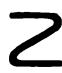
\includegraphics[keepaspectratio]{images/part001_c96515a7.jpg}}

命题 3 的推论表明，域 K 的每个扩张 E 都是包含在 E 中的有限生成扩张的定向并。显然，K 的每个有限次扩张 E 也是有限生成的，因为 E 的一组基（作为 K 上的向量空间）也是 E 在 K 上的一组生成族；我们稍后将看到其逆命题不成立。

\subsection{复合扩张}

设 E 和 F 是域 K 的两个扩张。所谓 E 和 F 的一个复合扩张，我们指的是任意三元组 \((L, u, v)\)，其中 L 是 K 的一个扩张，u 是 E 到 L 的一个 K-同态，v 是 F 到 L 的一个 K-同态，并且域 L 由 \(u(E) \cup v(F)\) 生成（参见图 1）。

\pandocbounded{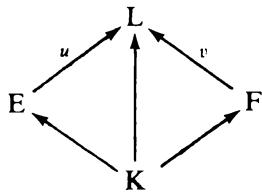
\includegraphics[keepaspectratio]{images/part001_6a404f81.jpg}}\\
图1。

按照一般定义（E，IV，第 6 页），E 和 F 的复合扩张 \((L, u, v)\) 到 E 和 F 的复合扩张 \((L', u', v')\) 上的一个同构是一个 K-同构 \(\varphi\)，它把 L 映到 \(L'\) 上，使得 \(u' = \varphi \circ u\) 且 \(v' = \varphi \circ v\) 。

设 \((\mathbf{L}, u, v)\) 是 \(\mathbf{E}\) 与 \(\mathbf{F}\) 的一个复合扩张。K-线性映射 \(w\)（从 \(\mathbf{E} \otimes_{\mathbf{K}} \mathbf{F}\) 到 \(\mathbf{L}\) 中）把 \(x \otimes y\) 映为 \(u(x)v(y)\)，它是一个 K-代数同态；在本节中，我们把它记作 \(u * v\) 。其像是 \(\mathbf{L}\) 中由 \(u(\mathbf{E}) \cup v(\mathbf{F})\) 生成的子环。

命题 4. --- 设 E、F 是 K 的两个扩张。

\begin{enumerate}
\def\labelenumi{\alph{enumi})}
\item
  设 \((\mathbf{L}, u, v)\) 是 \(\mathbf{E}\) 与 \(\mathbf{F}\) 的一个复合扩张；则 \(\mathfrak{p}\) 是一个素理想，它是同态 \(u * v\)（从 \(\mathbf{E} \otimes_{\mathbf{K}} \mathbf{F}\) 到 \(\mathbf{L}\) 中）的核。
\item
  设 \(\mathfrak{p}\) 是 \(E \otimes_{K} F\) 的一个素理想；则存在一个复合扩张 \((L, u, v)\) （\(E\) 与 \(F\) 的），使得 \(\mathfrak{p}\) 是 \(u * v\) 的核，且任意两个这样的复合扩张都是同构的。
\end{enumerate}

断言 a) 由环到域的同态的核是素理想这一事实得出（I，第 116-117 页）。

设 \(\mathfrak{p}\) 是 \(E \otimes_{K} F\) 的一个素理想，\(A\) 为商环 \((E \otimes_{K} F)/\mathfrak{p}\)，\(L\) 为 \(A\) 的分式域。对 \(x \in E\)（相应地 \(y \in F\)），我们用 \(u(x)\)（相应地 \(v(y)\)）表示在模 \(\mathfrak{p}\) 下 \(x \otimes 1\)（相应地 \(1 \otimes y\)）的剩余类。则 \(u\)（相应地 \(v\)）是 \(E\)（相应地 \(F\)）到 \(L\) 中的 K-同态，且 \(u(E) \cup v(F)\) 生成 \(A\)（作为环），因此生成 \(L\)（作为域）。因此 \((L, u, v)\) 是 \(E\) 与 \(F\) 的一个复合扩张；我们立刻看出 \(u * v\) 是 \(E \otimes_{K} F\) 到 \(L\) 中的典范同态，因此其核等于 \(\mathfrak{p}\) 。

设 \((L', u', v')\) 是 E 和 F 的一个复合扩张，使得 \(u' * v'\) 的核等于 p。由于 \(u * v\) 与 \(u' * v'\) 具有相同的核，存在一个同构 \(\psi\) ，它把 A 映到 \(u' * v'\) 的像 A' 上，由 \(u' * v' = \psi \circ (u * v)\) 刻画。但 A' 是由 \(u'(E) \cup v'(F)\) 生成的 L' 的子环，因此 \(L'\) 是 \(A'\) 的分式域。所以 \(\psi\) 扩张为一个同态 \(\varphi\) （把 L 映到 \(L'\) 上），并且显然 \(\varphi\) 是 \((L, u, v)\) 到 \((L', u', v')\) 上的一个同构。

注记。--- 若 p 和 \(p'\) 是 \(E \otimes_{K} F\) 的两个不同素理想，则对应的 E 与 F 的复合扩张（按上述证明的步骤构造）并不同构。然而，它们作为 K 的扩张仍可能同构（见 V，第 146 页，习题 2）。

推论. --- 存在 E 与 F 的复合扩张。

因为交换环 \(E \otimes_{K} F\) 不化为 0，则它有素理想：克鲁尔定理（I，第 104 页）证明了极大理想的存在性，且每个极大理想都是素理想。

我们可以如下更精确地表述这个推论。设 \((\mathrm{E}, u)\) 与 \((\mathrm{F}, v)\) 是 K 的两个扩张；选取交换环 \(E \otimes_{K} F\) 的一个极大理想 m，并令 \(L = (E \otimes_{K} F)/m\)；则 L 是 K 的一个扩张。对 \(x \in E\)，记 \(u'(x)\) 为 \(x \otimes 1 \mod m\) 的剩余类，并类似地，记 \(v'(y)\) 为 \(1 \otimes y \mod m\) 的剩余类（对所有 \(y \in F\)）。于是我们有以下域同态的交换图

\pandocbounded{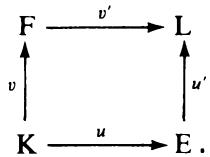
\includegraphics[keepaspectratio]{images/part001_e6455da9.jpg}}

通过把 \((L, u')\) 替换为 E 的一个同构扩张，我们可以假设 L 包含 E 作为子域，并且 \(u'\) 是 E 在 L 中的典范单射。通过更换记号，我们由此得到如下附注：

附注。--- 设 K 与 E 为两个域，且 u 为 K 到 E 的一个同态。若 K' 为包含 K 作为子域的域，则存在一个包含 E 作为子域的域 E'，以及 K' 到 E' 的一个同态 u'，它扩张 u。
